\documentclass[twoside,a4paper,11pt]{report}

%*******************************************************
% From page 7 of Preparing and Submitting Your
% Thesis - A guide for MPhil and PhD students:
% The thesis submitted for examination shall be typewritten
% or printed on one side or both sides of International size
% A4 paper (except for drawings, maps or tables on
% which no restriction is placed), with a margin of
% not less than 35mm on both right and left-hand
% edges of each page.
% There is no stipulation for the top and bottom margins,
% but it is recommended that they should be 25mm.
% From page10:
% Font heights are usually measured in points and
% the most easily readable fonts are 10 point and 12 point.
%*******************************************************

\usepackage[left=37mm,right=37mm,top=27mm,bottom=27mm]{geometry}

%*******************************************************
% Include packages that you wish to use.
%*******************************************************

\usepackage{tikz}
\usetikzlibrary{shapes,arrows}

\usepackage{lipsum} % this generates dummy text

\usepackage{multicol} % use multicolumn
\usepackage{rotating} % to create a figure in landscape mode

\usepackage{setspace} % this is for setting line spacing

\usepackage{longtable} % this is for longtable


\usepackage{array}


\usepackage{amsthm}
\usepackage{amsmath}
\usepackage{calc}
\usepackage{float}
\usepackage{graphicx}
\usepackage{setspace}
\usepackage{url}

\usepackage{nomencl}
\makenomenclature

%*******************************************************
% Define hyphenation for some special words
%*******************************************************

\usepackage{hyphenat} % this define hyphenation, an example is given in the next four lines.
\hyphenation{electro-magnets}

%*******************************************************
% Make "clickable" Table of Contents
%*******************************************************
\usepackage{color}   %May be necessary if you want to color links
\usepackage{hyperref}
\hypersetup{
    colorlinks=true, %set true if you want colored links
    linktoc=all,         %set to all if you want both sections and subsections linked
    linkcolor=blue,  %choose some color, e.g. blue, if you want links to stand out
    }

%*******************************************************
% This is the start of the thesis
%*******************************************************

\begin{document}

\linespread{1.2} % change it to 1 becomes single line spacing. Change it to 1.5 is a half line spacing.

%*******************************************************
% From page 10 of Preparing and Submitting Your Thesis
% A guide for MPhil and PhD students:
% Modern word processing programs will automatically
% adjust the line spacing to match the size of text on any line.
% Single line spacing will produce a dense but readable
% text: the text may seem less formidable if one and a
% spacing is used. Double spacing results in a rather
% empty looking page and significantly increases
% the number of pages in a thesis.
%*******************************************************

%*******************************************************
% These are front matters.
% Abstract
% Title page
% Declaration
% Acknowledgment
% Table of Contents (Including List of Tables and List of Figures)
% List of Abbreviations}
%*******************************************************

\pagenumbering{roman}
\pagestyle{plain}

%*******************************************************
% Abstract
%*******************************************************
\phantomsection
\addcontentsline{toc}{chapter}{Abstract}

\begin{center}

Abstract of thesis entitled\\

\bigskip

    \huge\textbf{Search for chargino and neutralino production in final states with two same-sign leptons, jets and missing transverse momentum at $\sqrt{s} = 13$ TeV with the ATLAS detector} \\

    \bigskip

    {\normalsize Submitted by}\\

\bigskip

    \Large{\textbf{Cheuk Yee LO}}\\

\bigskip

{\normalsize
for the degree of Doctor of Philosophy\\
at The University of Hong Kong\\
in November 2018\\}

\end{center}

\bigskip

The Standard Model in particle physics has successfully explained almost all experimental results in the microscopic scale with high accuracy.
However, the nature of dark matter and the Higgs mass hierarchy problem are still unanswered questions.
Supersymmetry (SUSY), which proposes a new symmetry between fermions and bosons, is one of the most promising theories beyond the Standard Model for potentially answering these questions.
In recent searches for supersymmetric particles that are involved in strong interaction, their masses were found to be above 1 TeV.
Since the production cross section drops as the masses of particles increase,
this might suggest that the pair production of electroweak gauginos, which tend to have lower mass, is a dominant SUSY production process at the Large Hadron Collider (LHC).
In addition, the upgrade in the increased center-of-mass energy of the proton-proton collisions $\sqrt{s}$ to 13 TeV has opened a new phase of exploration for electroweak SUSY productions.

In this thesis, a search is presented for the electroweak pair production of a chargino and a neutralino ($p + p \rightarrow \tilde{\chi}_1^\pm + \tilde{\chi}_2^0$),
where the chargino decays to the lightest neutralino and a W boson ($\tilde{\chi}_1^\pm \rightarrow \tilde{\chi}_1^0 + W$),
and the second lightest neutralino decays to the lightest neutralino and a Standard-Model-like Higgs boson ($\tilde{\chi}_2^0 \rightarrow \tilde{\chi}_1^0 + h$).
The final state with two same-sign leptons, jets and missing transverse momentum is considered in this search.
The two leptons come from the leptonic decay of the W boson and the Higgs boson, with the decay modes of  $h \rightarrow WW$, $h \rightarrow \tau \tau$ or $h \rightarrow ZZ$.
This analysis is based on the proton-proton collision data delivered by the LHC at $\sqrt{s}$ = 13 TeV with the ATLAS (A Toroidal LHC ApparatuS) particle detector.
The integrated luminosity of data is 36.1 fb$^{-1}$.

As a result, observations are consistent with the Standard Model predictions, therefore new exclusion limits for the masses of $\tilde{\chi}_1^\pm$/$\tilde{\chi}_2^0$ and $\tilde{\chi}_1^0$ are set, which supersedes the run 1 results.

\bigskip

\begin{center}

\rule{6cm}{0.025cm}\\
{\slshape An abstract of exactly 307 words}

\end{center}

%*******************************************************
% Titlepage
%*******************************************************
\phantomsection
\addcontentsline{toc}{chapter}{Title Page}

\begin{titlepage}
    \begin{center}
        \large
            \hfill
            \vfill
        \begingroup
            \huge\textsc{\textbf{This is the title of my thesis}} \\
            \bigskip
        \endgroup
        by\\
    \bigskip
        \Large\textsc{\textbf{Cheuk Yee LO}}\\
        \vfill
        \vfill
        \vfill
    {\normalsize
    A thesis submitted in partial fulfilment of the requirements for\\
    the Degree of Doctor of Philosophy\\
    at The University of Hong Kong.\\
        \bigskip
    August 2018}
        \vfill
        \end{center}
\end{titlepage}

%*******************************************************
% Declaration
%*******************************************************

\addcontentsline{toc}{chapter}{Declaration}

\chapter*{Declarations}

I declare that this thesis represents my own work, except where due acknowledgement is made, and that it has not been previously included in a thesis, dissertation or report submitted to this University or to any other institution for a degree, diploma or other qualifications.% This is copied from the declaration statement from the Handbook.

\bigskip
\bigskip
\bigskip
\bigskip
\bigskip
\bigskip
\bigskip
\bigskip

\begin{flushright}
    \begin{tabular}{p{2cm} p{4cm}}
        Signed & \dotfill \\
           & \center Cheuk Yee LO\\
    \end{tabular}
\end{flushright}

\bigskip
\bigskip
\bigskip

%*******************************************************
% Acknowledgments
%*******************************************************

\addcontentsline{toc}{chapter}{Acknowledgments}
\chapter*{Acknowledgments}

I would like to take this opportunity to thank some people who helped me do the research.

I would like to thank my supervisor Dr. Tu Yanjun for giving me the opportunity to do the research, for her support on my research and for her guidance and suggestions on my analysis.

I would like to thank Dr. Zhang Dongliang.
He taught me almost everything on the analysis.
He taught me the linux software: the linux shell, the text editor (vim) and the revision control system (svn).
He taught me the ATLAS software: the event analysis software (ROOT and RootCore), the data acquisition software(dq2 and rucio) and the distributed computing management (grid and panda).
He taught me the typesetting system (latex).
He taught me the ALTAS detector: trigger system and GRL.
He also helped our group to write the multiLepSearch package to generate the ntuple.

I would like to thank Dr. Daniela Paredes.
She gave a lot of suggestions on my analysis.
She also helped our group to do analysis.



%*******************************************************
% This program is free software: you can redistribute it and/or modify
% it under the terms of the GNU General Public License as published by
% the Free Software Foundation, either version 3 of the License, or
% (at your option) any later version.
%
% This program is distributed in the hope that it will be useful,
% but WITHOUT ANY WARRANTY; without even the implied warranty of
% MERCHANTABILITY or FITNESS FOR A PARTICULAR PURPOSE.  See the
% GNU General Public License for more details.
%
% You should have received a copy of the GNU General Public License
% along with this program.  If not, see <http://www.gnu.org/licenses/>.
%*******************************************************
% Table of Contents
%*******************************************************


\setcounter{tocdepth}{2} % <-- 2 includes up to subsections in the ToC
\setcounter{secnumdepth}{3} % <-- 3 numbers up to subsubsections

\tableofcontents 

%*******************************************************
% List of Figures and of the Tables
%*******************************************************

\clearpage

\listoffigures

\cleardoublepage
 
\listoftables

\cleardoublepage

\clearpage
\phantomsection
\addcontentsline{toc}{chapter}{List of Abbreviations and Symbols}

\nomenclature{SM}{Standard Model}
\nomenclature{BSM}{beyond the Standard Model}
\nomenclature{SUSY}{Supersymmetry}
\nomenclature{LHC}{Large Hadron Collider}
\nomenclature{lepton}{refer to electron or muon}
\nomenclature{jet}{a particle shower in a narrow cone from the hadronization of a quark or a gluon}

\nomenclature{MC}{Monte Carlo Simulation}
\nomenclature{Data}{the experimental data}
\nomenclature{BG}{background}

\nomenclature{SR}{signal region}
\nomenclature{CR}{control region}
\nomenclature{VR}{validation region}

\nomenclature{N-1 plot}{The plot with all selections are applied, except the cut of that variable}
\nomenclature{yield}{The resulting number of events}

\nomenclature{SS}{same sign}
\nomenclature{OS}{opposite sign}

\nomenclature{$p_T$}{transverse momentum}
\nomenclature{$\eta$}{pseudorapidity}

\renewcommand{\nomname}{List of Abbreviations and Symbols}
\printnomenclature


%*******************************************************
% Mainmatter
%*******************************************************

\pagenumbering{arabic}

\cleardoublepage
%************************************************
\chapter{Experimental Setup}
\label{ch:detector}
%************************************************

\section{Introduction}
\label{sec:detector_introduction}

Our experimental data was collected from the ATLAS particle detector in the Large Hadron Collider (LHC).
The following section will introduce LHC and the ATLAS particle detector.

\section{The Large Hadron Collider}
\label{sec:detector_LHC}

The Large Hadron Collider (LHC) was built in the border between France and Switzerland by the European Organization for Nuclear Research (CERN).
It is a circular particle collider under the ground with circumference 27 km.
Two beams of protons will be accelerated in opposite directions, and then these two beams will collide with each other at the collision point.
The energy of each beam is 6.5 TeV, and hence the center-of-mass energy of the two beams $\sqrt{s}$ is 13 TeV, which is the energy used in this experiment.
This energy is equivalent to the speed that the beam will circulate the ring 11,245 times per second.
Figure \ref{fig:detector_LHC_accelerator_complex} shows the schematic diagram of the CERN accelerator complex, which contains a series of accelerators, from low energy to high energy.
The dark blue big circle in figure \ref{fig:detector_LHC_accelerator_complex} represents the LHC, on which there are 4 particle detectors at 4 different yellow points: ATLAS, CMS, LHCb and ALICE.

\begin{figure}
\centering
\includegraphics[width=\textwidth]{data/photo/accelerator_complex.png}
\caption{The schematic diagram of the CERN accelerator complex, which shows a series of accelerators and facilities. \cite{complex}}
\label{fig:detector_LHC_accelerator_complex}
\end{figure}

Before the beam is injected into LHC, the protons need to be accelerated by a series of accelerators.
The journey of the protons starts from a tank of hydrogen gas.
The proton and the electron are separated by a electric field.
The protons are then accelerated to 50 MeV by Linac2, which is a linear accelerator.
The beam is then injected to the second accelerator called the Proton Synchrotron Booster (PSB), which accelerates the beam to 1.4 GeV.
The beam is then injected to the third accelerator called the Proton Synchrotron (PS), which pushes the beam to 25 GeV.
The beam is then injected to the fourth accelerator called the Super Proton Synchrotron (SPS), which further pushes the beam to 450 GeV.
Finally, the beam is injected to the two beam pipes of the LHC.
One of the beam moves in clockwise direction, while another beam moves in anti-clockwise direction.
Two beams will be collided at the collision point inside the ATLAS detector.
\cite{accelerator}

The circular path of the proton beam is maintained by many superconducting electromagnets along the LHC tunnel.
There are 1232 main magnetic dipoles, and each of them generates a large magnetic field of 8.3 T.
In order to generate such a high magnetic field, the coils need to have very high currect of 11,080 A, and hence supercoducting coil need to be used, to reduce the heat loss due to the electrical resistance.
The material of supercoducting coil is niobium-titanium (NbTi).
To reach the condition for supercoductivity, the electromagnets operate at a very low temperature of 1.9 K.
There are also 392 magnetic quadrupole to make the beam narrower, and the chance of proton-proton collision will be higher.
\cite{supermagnet,cryogenics}

The protons in the beam are grouped into different bunches, and there are about $10^{11}$ protons in each bunch.
The time-spacing between two adjacent bunches is 25ns (or 50 ns in the old configuration).
This means that in each 25 ns, two bunches are collided at the collision point.
For each bunch collision, there are about 10 to 50 proton-proton interaction.

The interacting rate for a physics proccess $\frac{dN}{dt}$ is the product of the cross section of that physics proccess $\sigma$ and the instantaneous luminosity $\mathcal{L}$.
\begin{equation}
\frac{dN}{dt} = \sigma \mathcal{L}
\end{equation}
The instantaneous luminosity $\mathcal{L}$ is a measure of the interacting rate of two protons at the collision point, which is related to the density of the protons and the speed of the protons.
The instantaneous luminosity in this experiment is about $10^{34}$ cm$^{-2}$ s$^{-1}$ (or 10 nb$^{-1}$ s$^{-1}$).

\section{ATLAS detector}
\label{sec:detector_ATLAS}

A Toroidal LHC ApparatuS (ATLAS) is the particle detector used in this experiment \cite{ATLAS_doc}.
Figure \ref{fig:detector_ATLAS} shows the main components of the ATLAS detector.
\begin{figure}
\centering
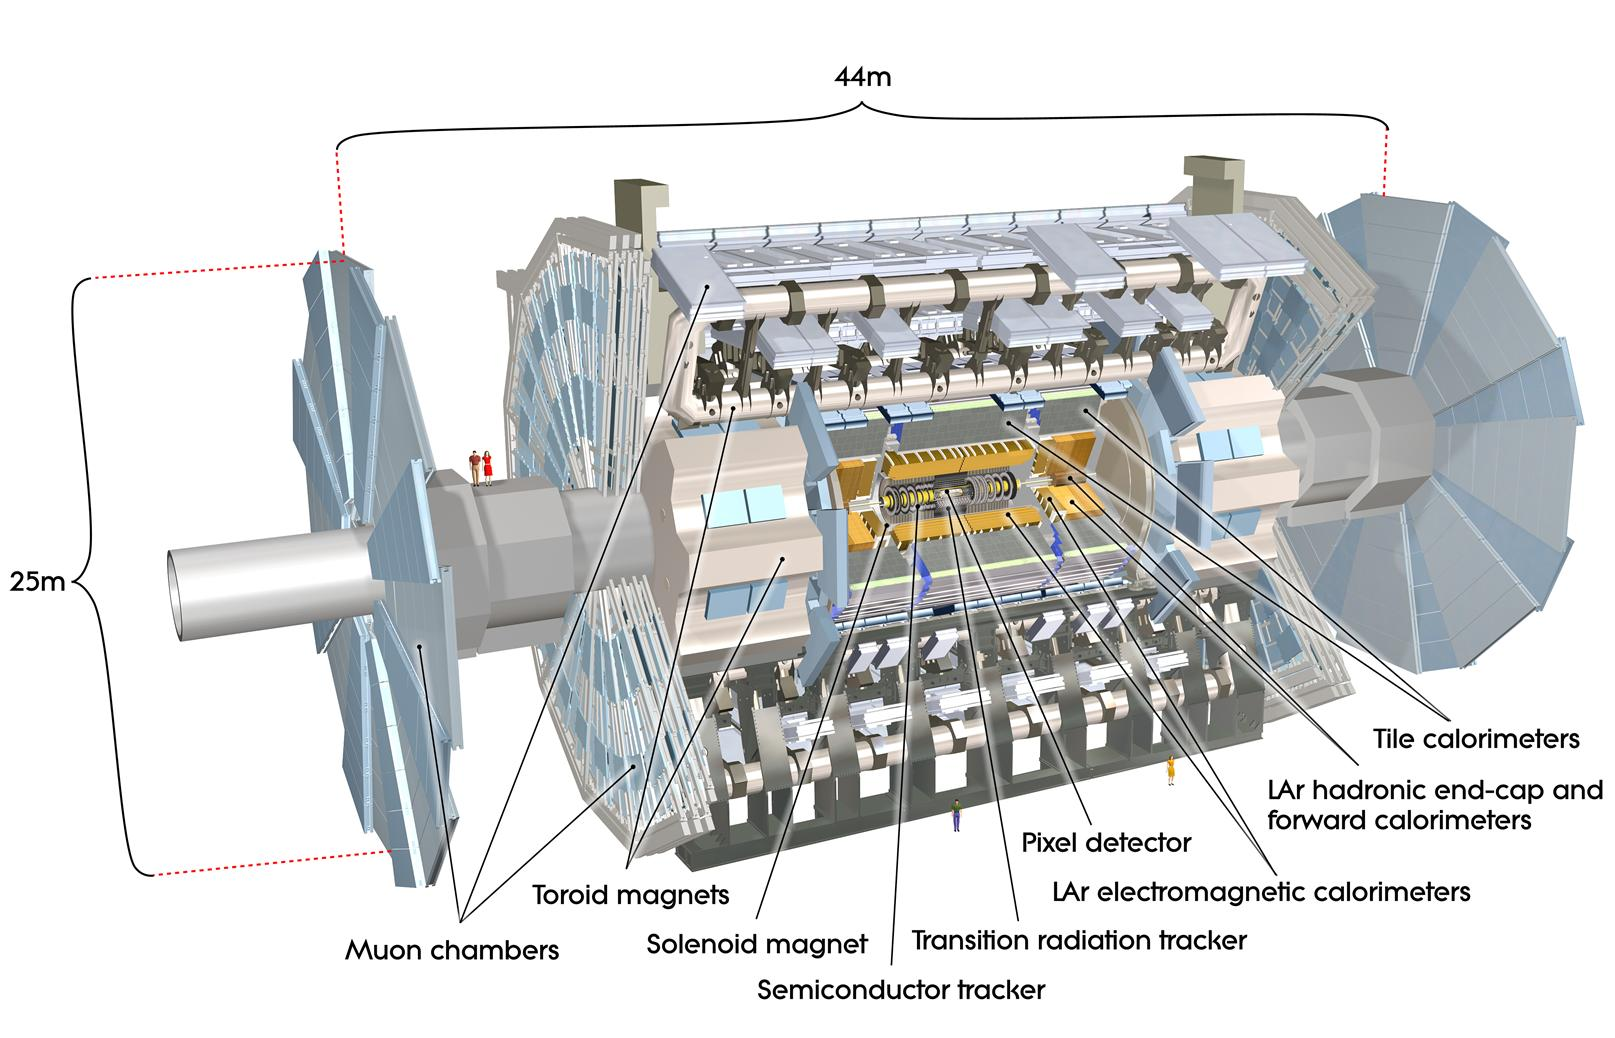
\includegraphics[width=\textwidth]{data/photo/ATLAS.jpg}
\caption{The cut-away view of the ATLAS detector. It is 25m high and 44m long. \cite{ATLAS_photo}}
\label{fig:detector_ATLAS}
\end{figure}
The ATLAS detector is a general purpose particle detector, which is consisted of 3 main components: the inner detector, the calorimeter and the muon spectrometer.
Figure \ref{fig:ATLAS_particles} shows how the ATLAS distinguishes different types of particle. The inner detector can detect the paths of the charged particles.
Photons and electrons will deposit most of their energy in the electromagnetic calorimeter, and finally stop by it.
Hadrons(including protons and neutrons) and mesons will similarly stop by the hadronic calorimeter.
Only muons and the neutrinos can reach the outermost muon spectrometer, but only muons can be detected by the muon spectrometer.
Nearly all neutrinos will escape the whole ATLAS detector, which leads to some missing energy.
In this design, different particles can be identified due to their signature in different parts of ATLAS.
\begin{figure}
\centering
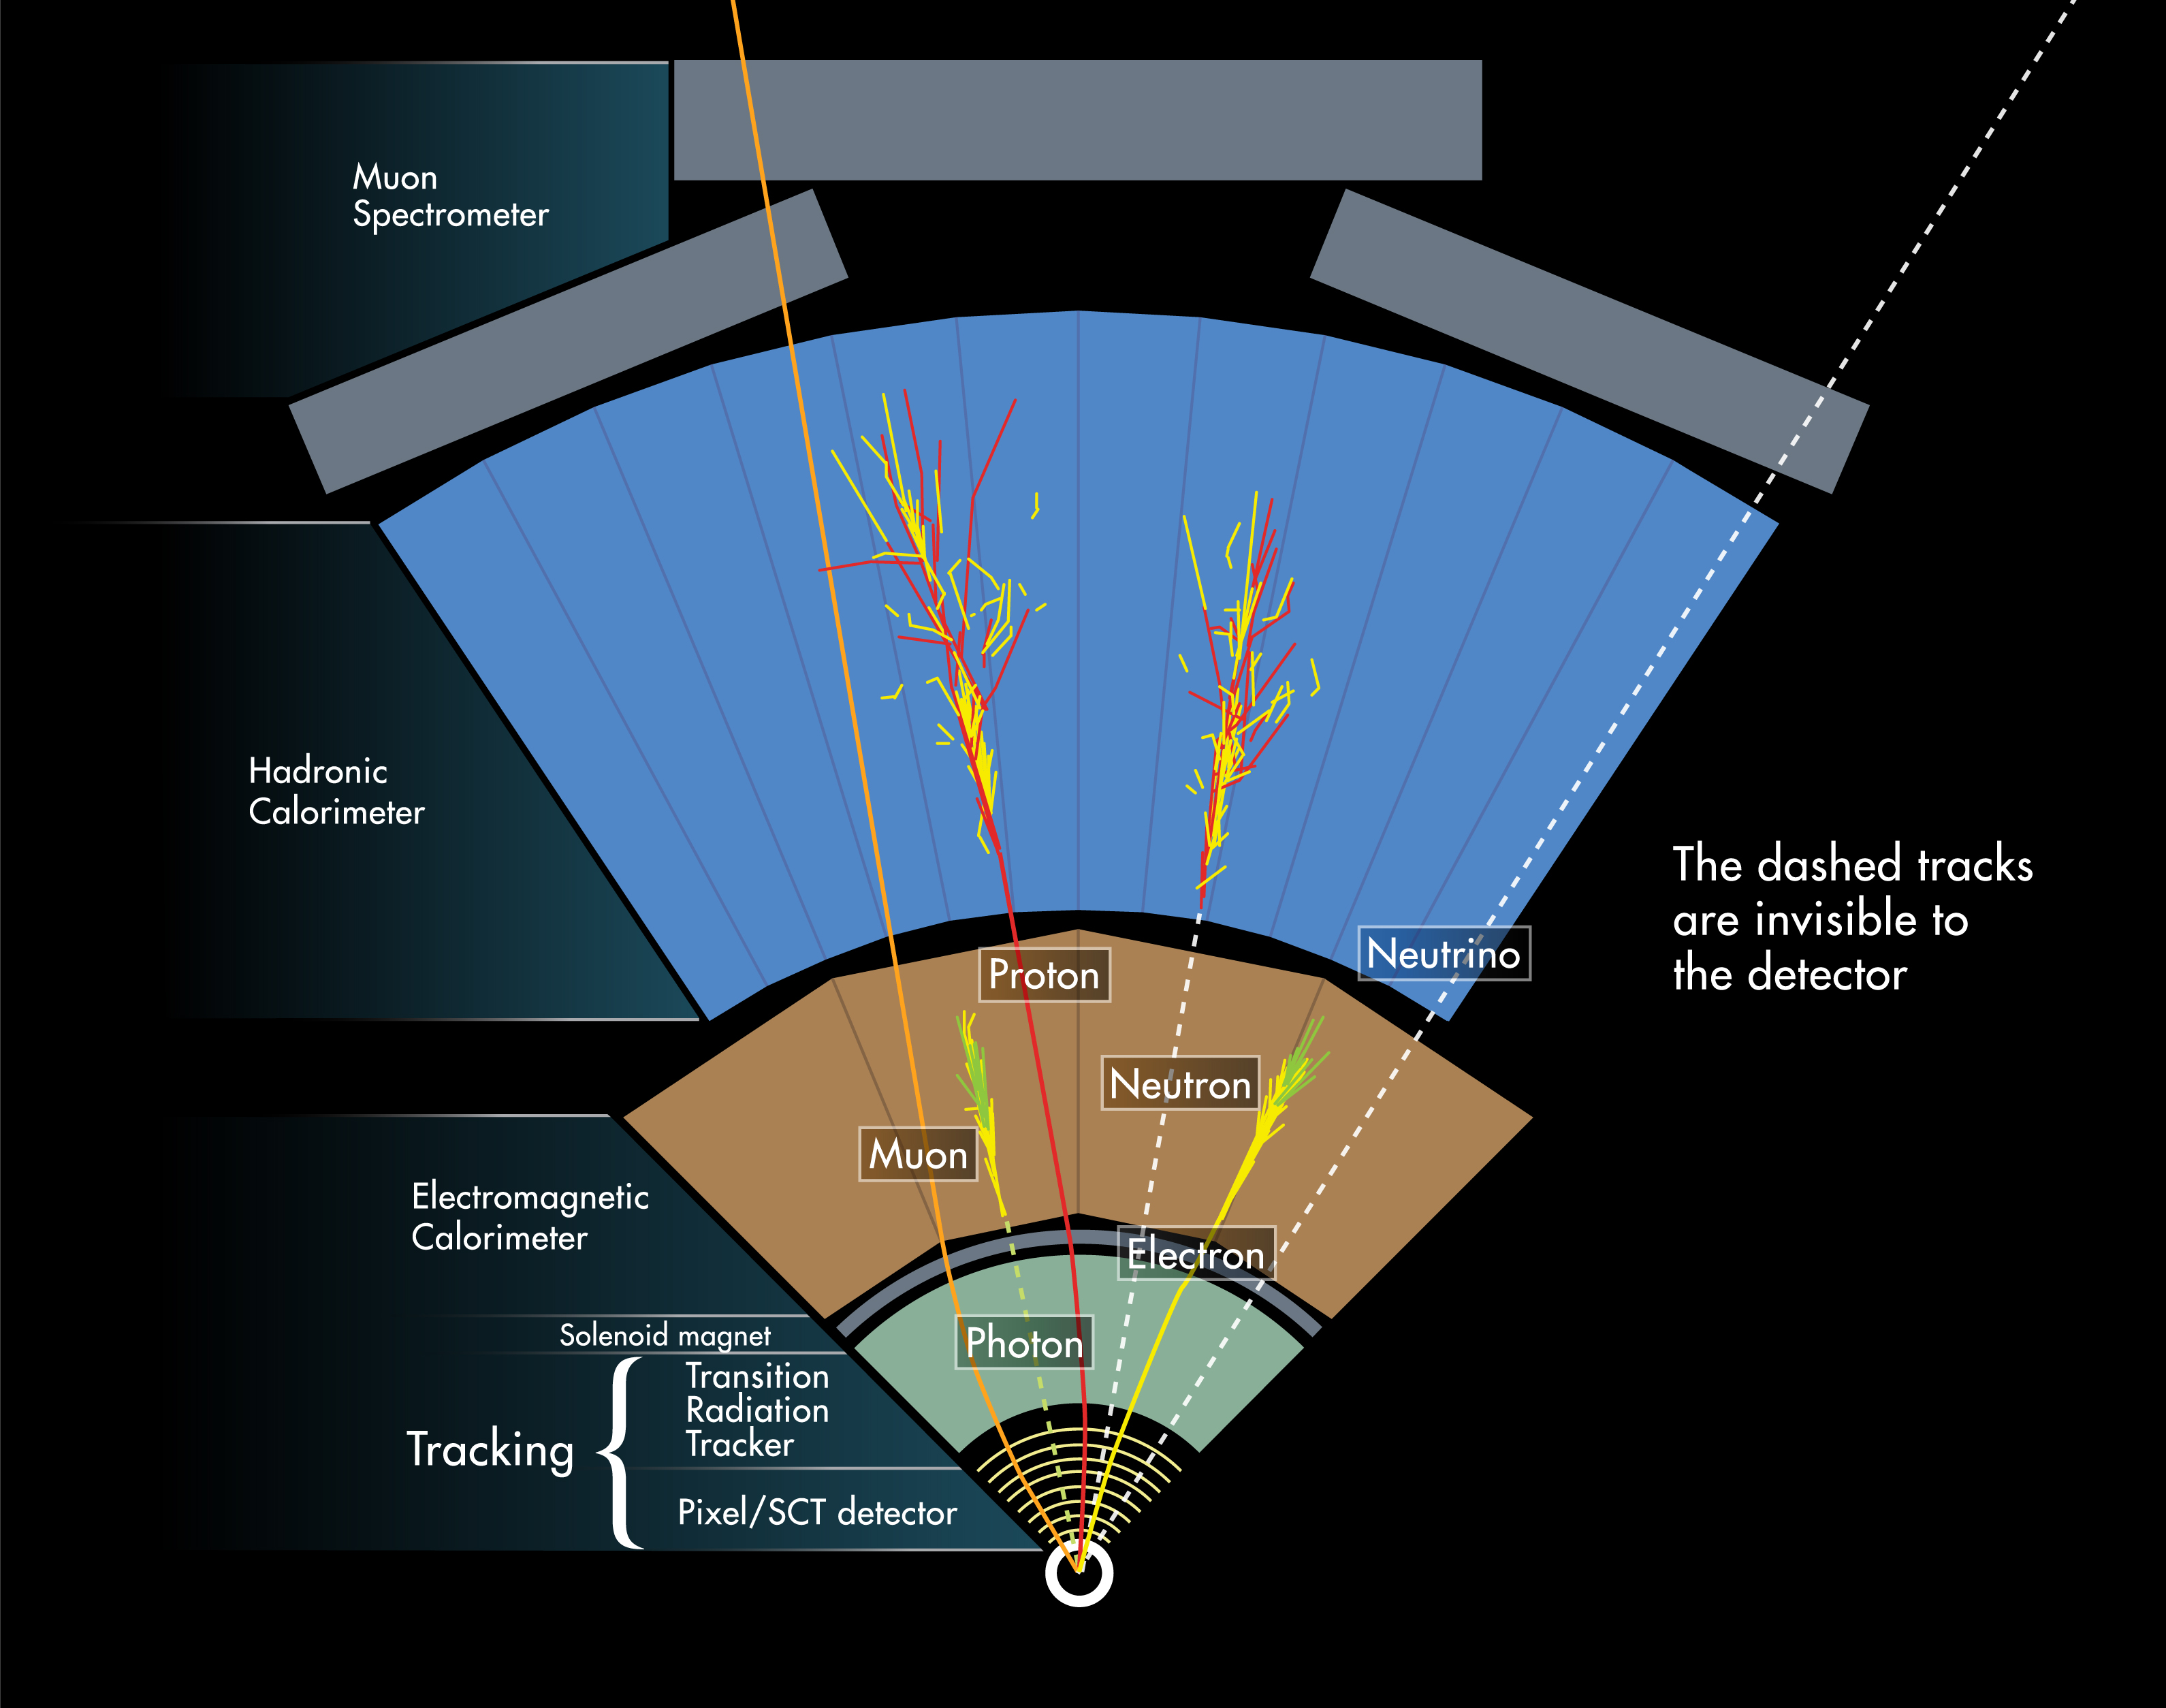
\includegraphics[width=\textwidth]{data/photo/ATLAS_particles.jpg}
\caption{The cross section of the ATLAS detector. This shows different components of the ALTAS and how ATLAS detect different types of particles \cite{ATLAS_particles}}
\label{fig:ATLAS_particles}
\end{figure}

\subsection{coordinate system}
The nominal collision point is defined as the origin of the coordinate system.
The z-axis is along the beam dirention.
The positive x-asix is pointing to the centre of the LHC ring.
The positive y-asix is in the upward direction.
The azimuthal angle $\phi$ and the polar angle $\theta$ are defined as usual in the spherical coordinate system.
The pseudorapidity $\eta$ is defined as:
\begin{equation}
\eta = - \ln \Big( \tan \frac{\theta}{2} \Big)
\end{equation}
The distance $\Delta R$ in the pseudorapidity-azimuthal angle space is defined as:
\begin{equation}
\Delta R = \sqrt{(\Delta \phi) ^2 + (\Delta \eta) ^2}
\end{equation}
The ATLAS detector has a reflection symmetry about the x-y plane.

\subsection{magnetic system}
There is a thin superconducting solenoid magnet around the inner detector, which generates a 2 T magnetic field inside the inner detector.
There are also 3 large superconducting toroids around the calorimeter: one for barrel and two for end-caps.
All these magnets are shown in figure \ref{fig:detector_ATLAS}.

\subsection{The inner detector}
The inner detector is a particle tracker.
It mainly detects the tracks of charged particles and has good performance for measuring the momentum of the charged particles and locating the position of the vertices.
Figure \ref{fig:detector_inner_whole} shows the whole structure of the inner detector.
The inner detector consists of 3 sub-detectors from inner to outer: the pixel detector, the silicon microstrip tracker (SCT) and the transition radiation tracker (TRT).
Each part further divides into two parts: the barrel region with smaller $|\eta|$ and the end-cap region with larger $|\eta|$.
Figure \ref{fig:detector_inner_detail} shows the distances R from the beam for the 3 sub-detectors, and figure \ref{fig:detector_inner_size} shows the shapes and the orientations of each sensor and the $\eta$ coverage, in both the barrel and the end-cap regions.
The $\eta$ coverage for the inner detector is $|\eta| < 2.5$.
The shapes and the orientations of the sensors are different in the barrel and the end-cap regions.
In the barrel region, the shape and the orientation of the sensors is concentric cylinder shells around the beam axis, while in the end-cap region, they are disks perpendicular to the beam axis.
\begin{figure}
\centering
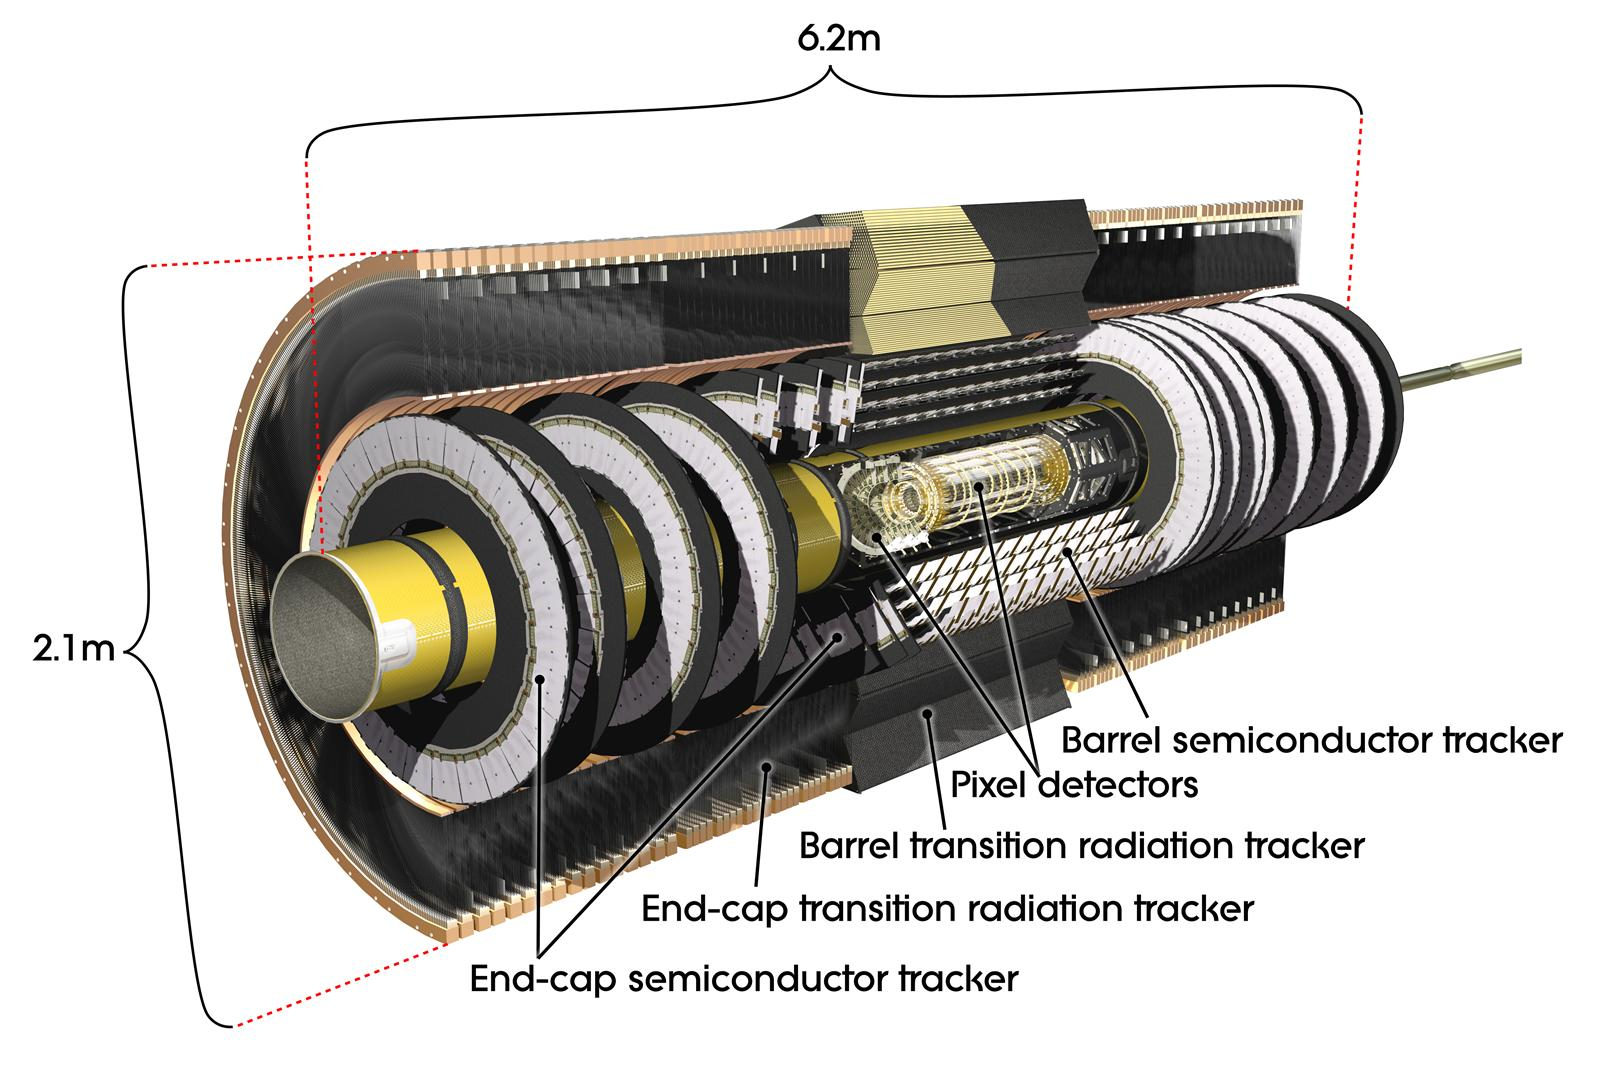
\includegraphics[width=\textwidth]{data/photo/inner_whole.jpg}
\caption{The whole structure of the ATLAS inner detector. \cite{inner_photo}}
\label{fig:detector_inner_whole}
\end{figure}
\begin{figure}
\centering
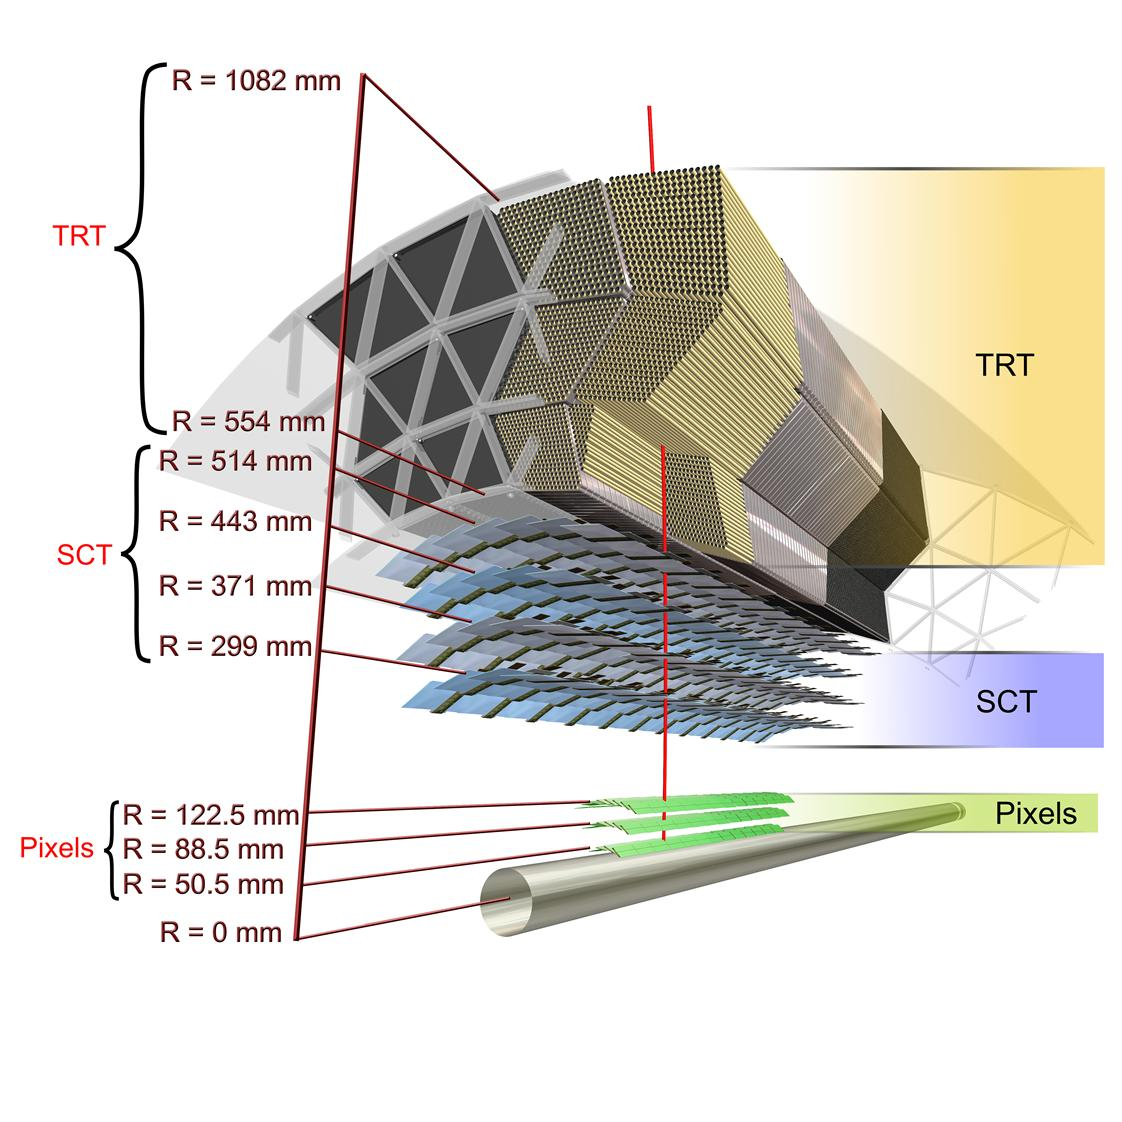
\includegraphics[width=\textwidth]{data/photo/inner_detail.jpg}
\caption{The distances R from the beam for the 3 components: pixel, SCT and TRT. \cite{inner_photo}}
\label{fig:detector_inner_detail}
\end{figure}
\begin{figure}
\centering
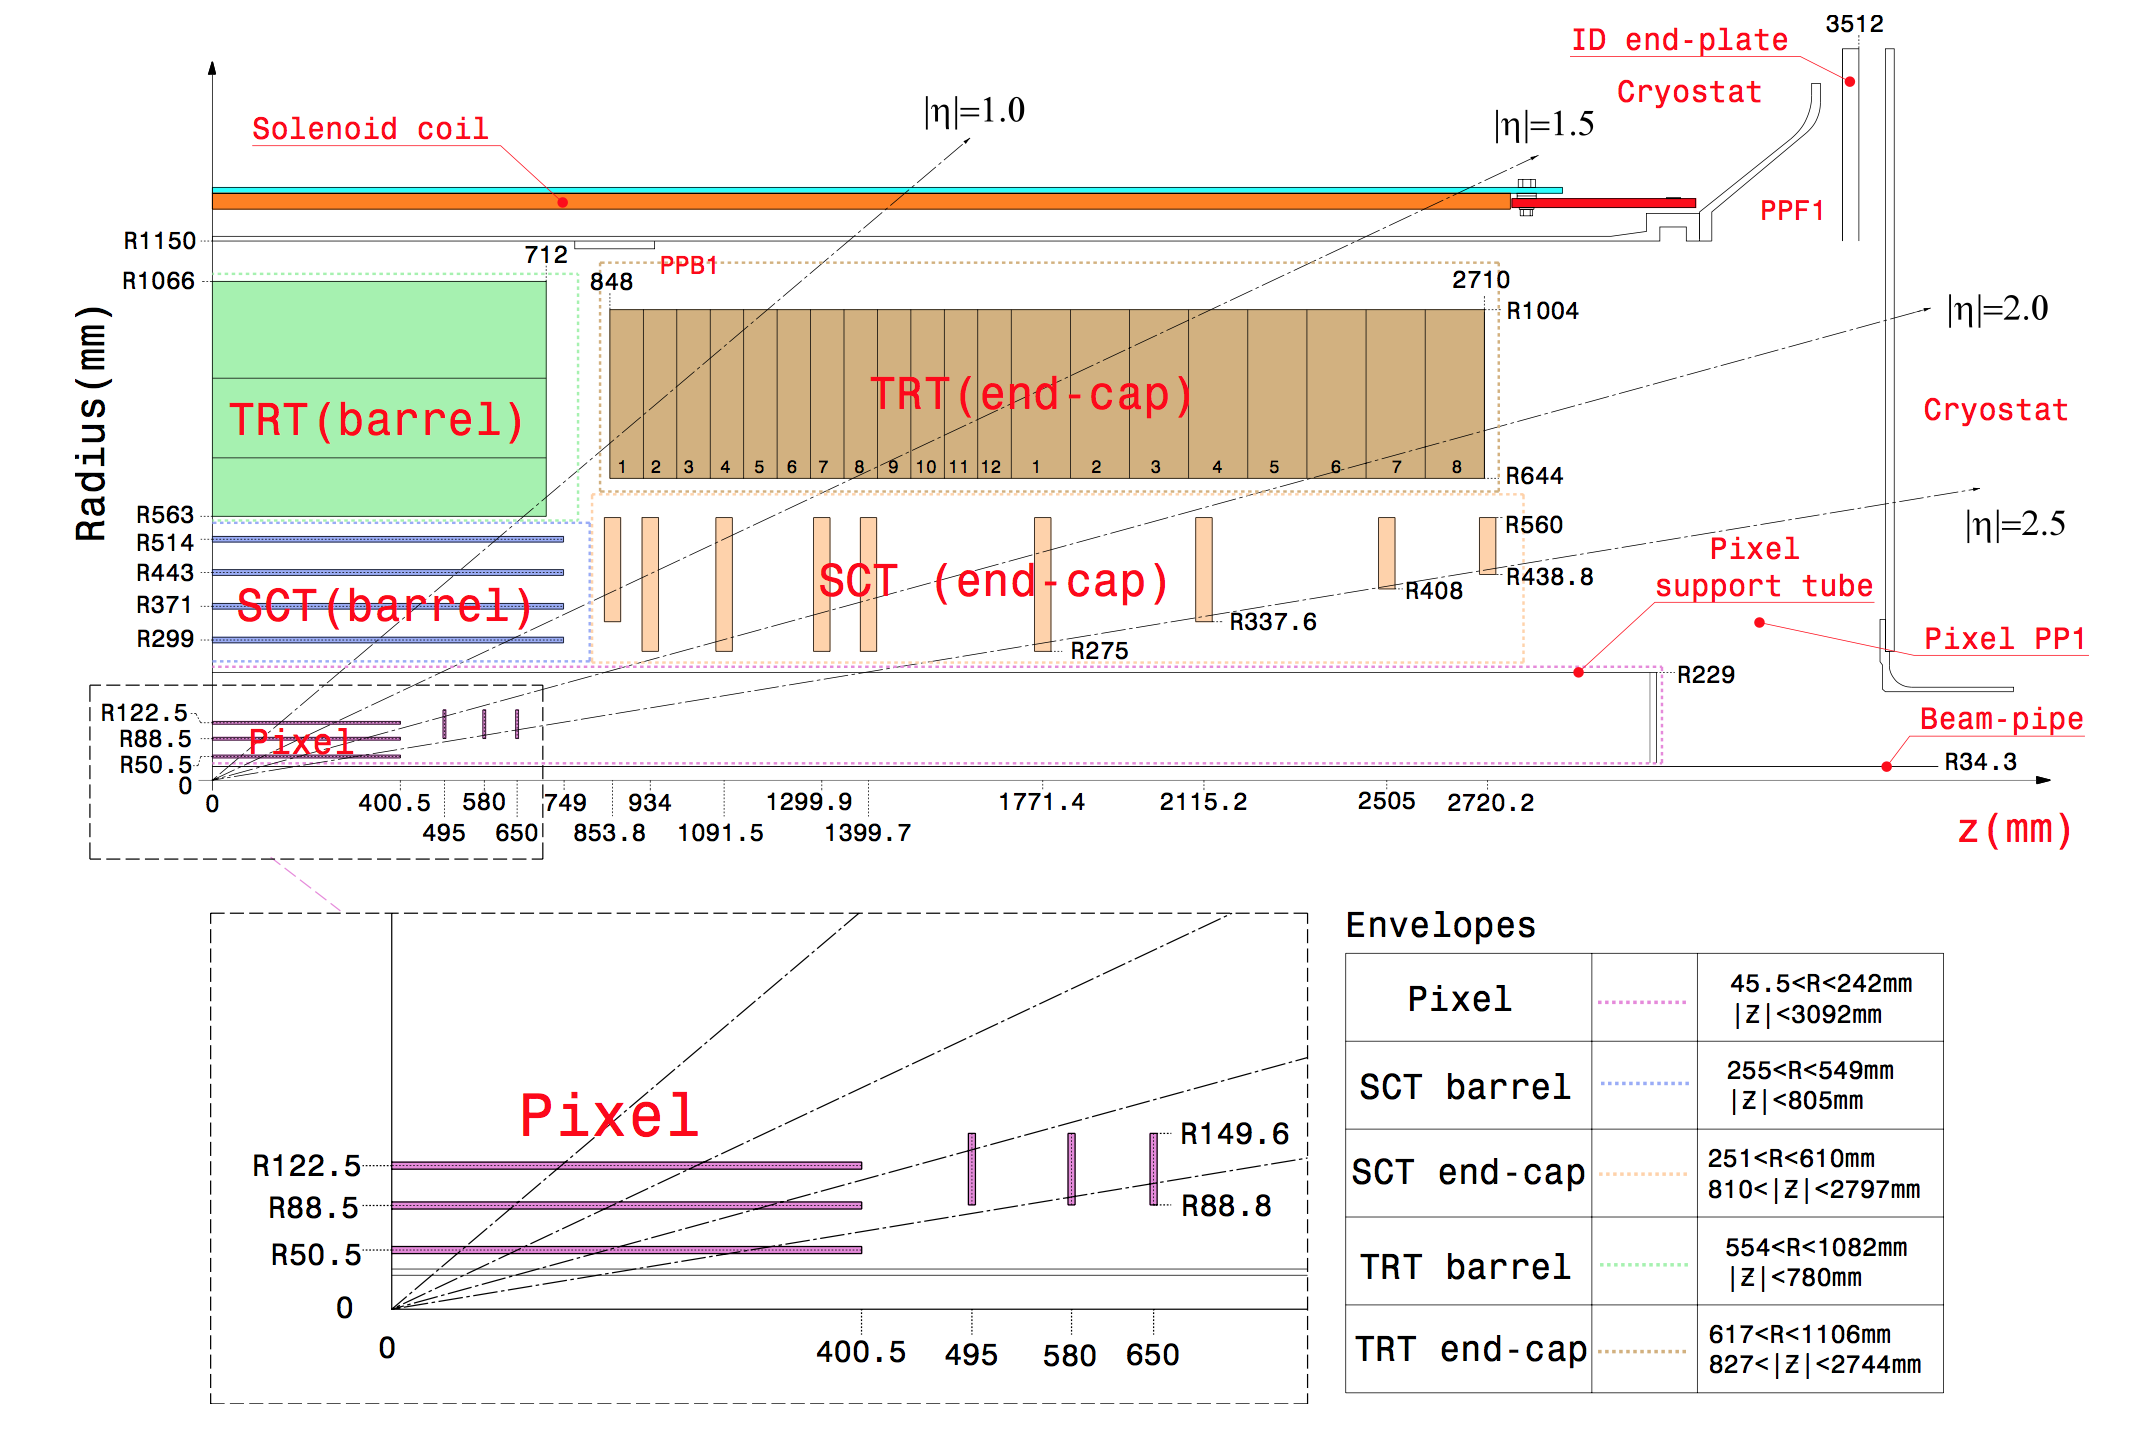
\includegraphics[width=\textwidth]{data/photo/inner_size.png}
\caption{The shapes, the orientations and the $\eta$ coverage for each sensor. \cite{ATLAS_doc}}
\label{fig:detector_inner_size}
\end{figure}

The precision tracking detectors (pixels and SCT) has high resolution in space by using discrete space-points to detect the track of a charged particle, with the cutting-edge technology, in order to achieve the good performance of the inner detector.
When the particle moves inside the inner detector, there are, in average, 36 hits per one track.
By recording the positions of these hits, the path of the particle can be reconstructed.
The whole inner detector is immersed in a 2 T magnetic field generated by the solenoid magnet, and hence the path of any charged particles will be bent.
By measuring the curvature of the path, the charge and momentum of the particle can be measured.
The equation for the circular path is
\begin{equation}
\frac{d\mathbf{p}}{dt} = q(\mathbf{v} \times \mathbf{B})
\end{equation}
where the relativistic momentum $\mathbf{p} = \gamma m \mathbf{v}$.
\begin{align}
\frac{d\mathbf{p}}{dt} &= q( \frac{\mathbf{p}}{\gamma m} \times \mathbf{B}) \\
&= \frac{q}{\gamma m} (\mathbf{p} \times \mathbf{B})
\end{align}
From this equation, we can get the angular frequence $\omega$,
\begin{align}
\omega &= \frac{qB}{\gamma m} \\
\frac{v}{r} &= \frac{qB}{\gamma m} \\
\frac{1}{r} &= \frac{qB}{\gamma m v} \\
\frac{1}{r} &= \frac{qB}{p} \\
p &= rqB
\end{align}
By this equation, we can calculate the momentum of the particle, from the curvature of track $1/r$, the charge and the magnetic field strength.

\subsubsection{Pixel detector}
As shown in figure \ref{fig:detector_inner_size}, there are 3 layers of cylinder in the barrel region, and 3 layers of disk for each end-cap region.
There are in total 1744 modules in the pixel detectors.
Each module is identical, and has the size of 19mm$\times$63mm, and 250 $\mu$m thick.
The module has 47232 pixels, which has size of 50$\mu$m$\times$400$\mu$m, and hence there are in total 80 million pixels for the whole pixel detector.
Each pixel has the accuracy of 10$\mu$m$\times$115$\mu$m.
The sensor is using planar n$^{+}$-in-n type of silicon, with n$^{+}$-type at the readout side and n-type at another side.

\subsubsection{SCT}
As shown in figure \ref{fig:detector_inner_size}, there are 4 layers of cylinder in the barrel region, and 9 layers of disk for each end-cap region.
There are in total 4088 modules in the SCT, with the thickness of 285 $\mu$m.
There are in total 6.3 million pixels for the SCT.
Each pixel has the accuracy of 17$\mu$m$\times$580$\mu$m.
The sensor is using planar p-in-n type of silicon.

\subsubsection{TRT}
136 TRT modules.
TRT in the outer part is to produce and detect the transition radiation from the particle. TRT comprises many layers of gaseous straw tube elements interleaved with transition radiation material.
Each pixel has the accuracy of 130$\mu$m.

\subsection{Calorimeter}
\begin{figure}
\centering
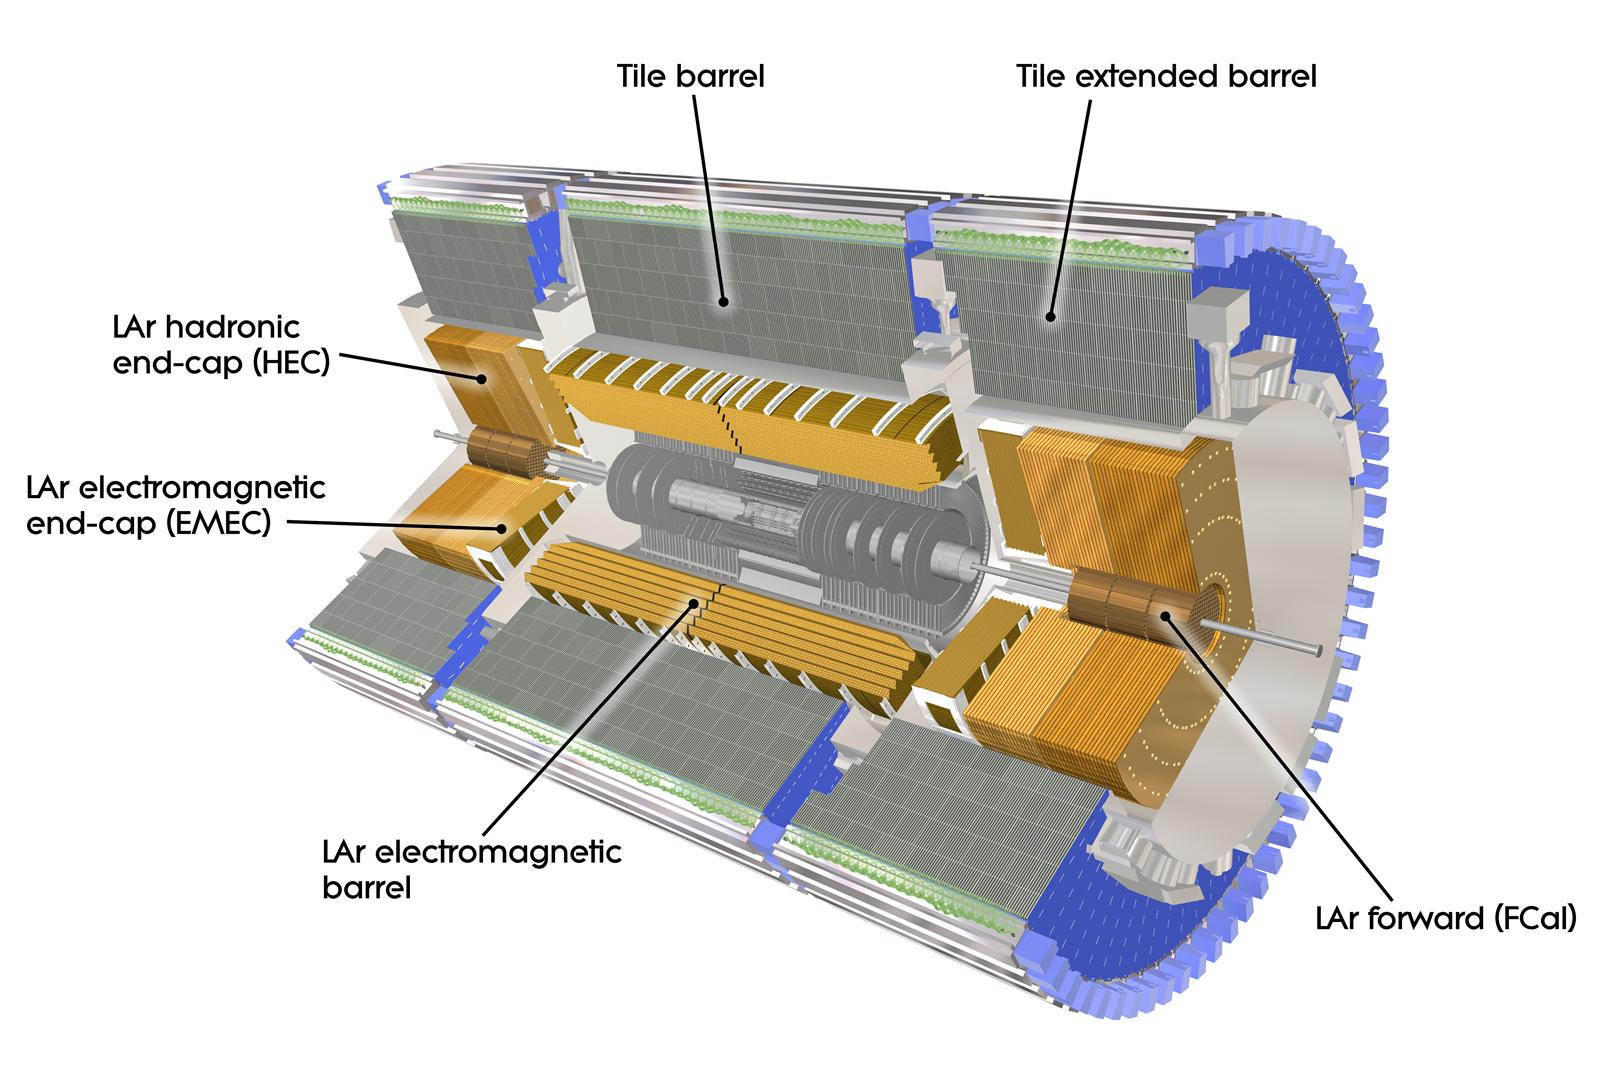
\includegraphics[width=\textwidth]{data/photo/calorimeter_whole.jpg}
\caption{whole calorimeter \cite{calorimeter_whole}}
\label{fig:calorimeter_whole}
\end{figure}

\subsubsection{Electromagnetic calorimeter}

\subsubsection{Hardronic calorimeter}

\subsection{Muon Spectrometer}
\begin{figure}
\centering
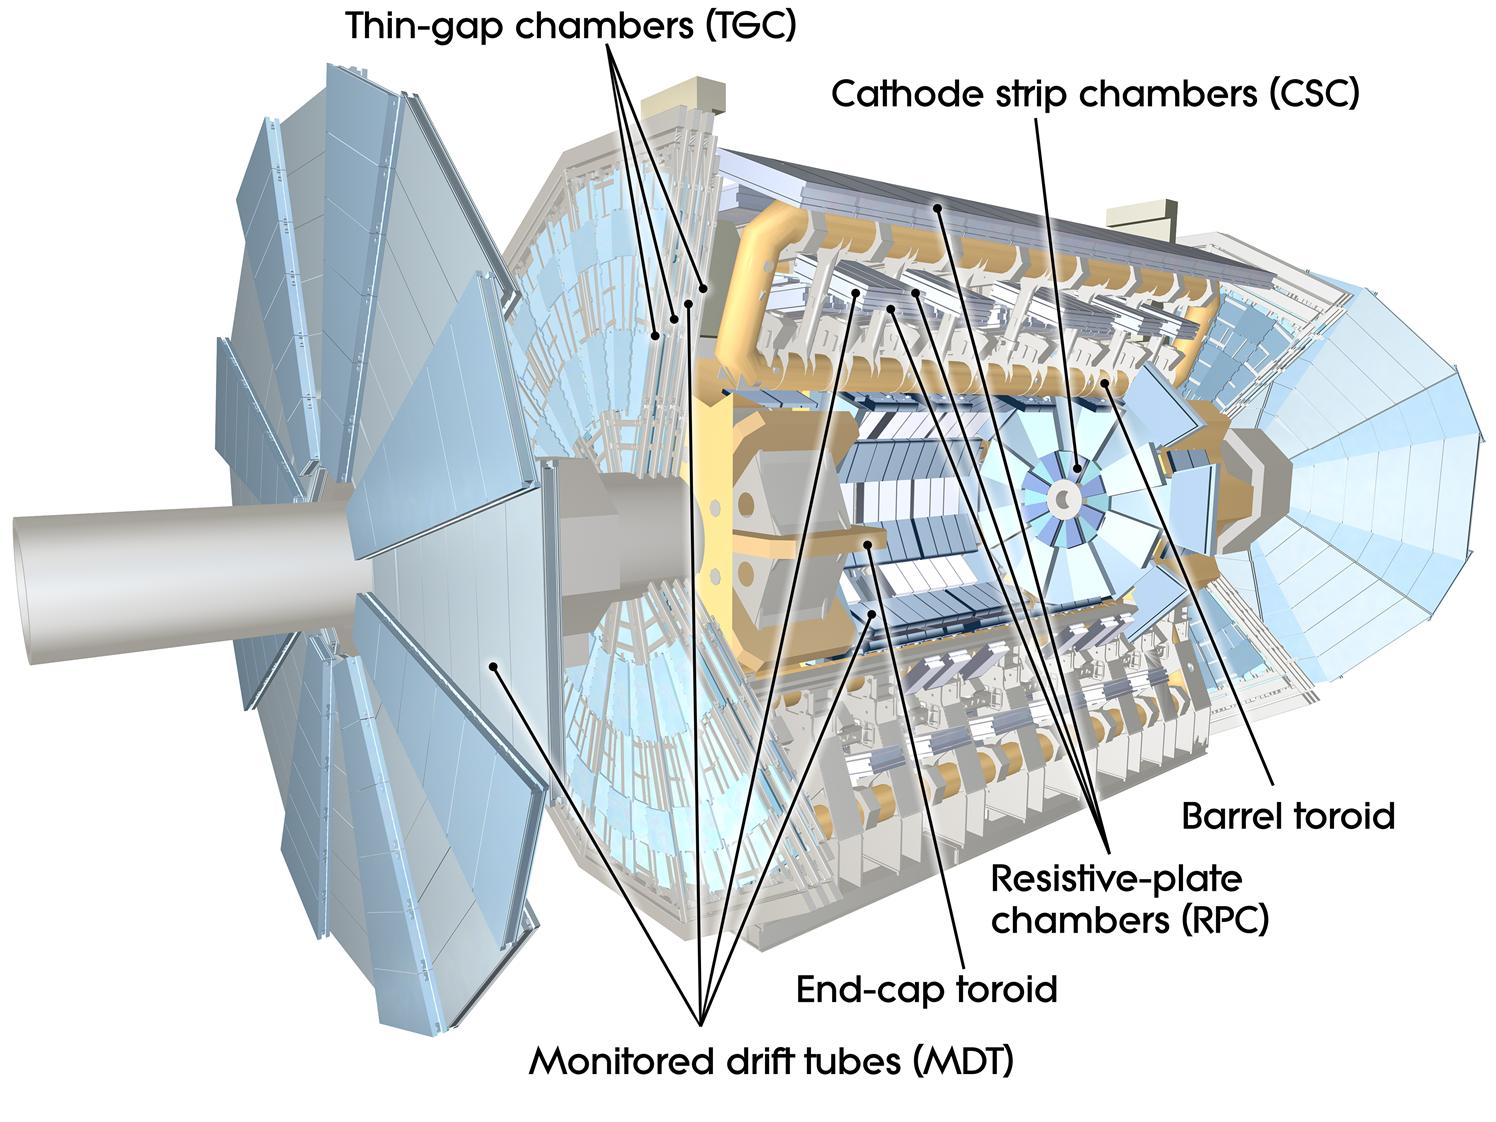
\includegraphics[width=\textwidth]{data/photo/muon_spectrometer.jpg}
\caption{muon spectrometer \cite{muon_spectrometer}}
\label{fig:muon_spectrometer}
\end{figure}


%*******************************************************
% Appendix
%*******************************************************

%\appendix
%%************************************************
\chapter{List of MC samples}
\label{ch:appendixOne}
%************************************************

\section{List of background MC samples}
\label{sec:MCBG}
\begin{table}[htbp]
\begin{center}
\tiny
\scalebox{0.7}{
\begin{tabular}{ccccccc}
\hline
Dataset ID & Process & Tags & Cross section [pb] & $k$-factor & Generator efficiency & $ \mathcal{L}_{int} [\mathrm{fb}^{-1}]$ \\
\hline
364156 & Sherpa\_221\_NNPDF30NNLO\_Wmunu\_MAXHTPTV0\_70\_CVetoBVeto & e5340\_s2726\_r7772\_r7676\_p2949 & 19143.0000 & 0.97 & 0.824 & 1.616 \\ 
364157 & Sherpa\_221\_NNPDF30NNLO\_Wmunu\_MAXHTPTV0\_70\_CFilterBVeto & e5340\_s2726\_r7772\_r7676\_p2949 & 19121.0000 & 0.97 & 0.130 & 4.071 \\ 
364158 & Sherpa\_221\_NNPDF30NNLO\_Wmunu\_MAXHTPTV0\_70\_BFilter & e5340\_s2726\_r7772\_r7676\_p2949 & 19135.0000 & 0.97 & 0.044 & 21.032 \\ 
364159 & Sherpa\_221\_NNPDF30NNLO\_Wmunu\_MAXHTPTV70\_140\_CVetoBVeto & e5340\_s2726\_r7772\_r7676\_p2949 & 944.8500 & 0.97 & 0.675 & 23.912 \\ 
364160 & Sherpa\_221\_NNPDF30NNLO\_Wmunu\_MAXHTPTV70\_140\_CFilterBVeto & e5340\_s2726\_r7772\_r7676\_p2949 & 937.7800 & 0.97 & 0.235 & 46.173 \\ 
364161 & Sherpa\_221\_NNPDF30NNLO\_Wmunu\_MAXHTPTV70\_140\_BFilter & e5340\_s2726\_r7772\_r7676\_p2949 & 944.6300 & 0.97 & 0.076 & 283.269 \\ 
364162 & Sherpa\_221\_NNPDF30NNLO\_Wmunu\_MAXHTPTV140\_280\_CVetoBVeto & e5340\_s2726\_r7772\_r7676\_p2949 & 339.5400 & 0.97 & 0.626 & 47.919 \\ 
364163 & Sherpa\_221\_NNPDF30NNLO\_Wmunu\_MAXHTPTV140\_280\_CFilterBVeto & e5340\_s2726\_r7772\_r7676\_p2949 & 340.0600 & 0.97 & 0.289 & 77.568 \\ 
364164 & Sherpa\_221\_NNPDF30NNLO\_Wmunu\_MAXHTPTV140\_280\_BFilter & e5340\_s2726\_r7772\_r7676\_p2949 & 339.5400 & 0.97 & 0.109 & 686.449 \\ 
364165 & Sherpa\_221\_NNPDF30NNLO\_Wmunu\_MAXHTPTV280\_500\_CVetoBVeto & e5340\_s2726\_r7772\_r7676\_p2949 & 72.0670 & 0.97 & 0.546 & 129.289 \\ 
364166 & Sherpa\_221\_NNPDF30NNLO\_Wmunu\_MAXHTPTV280\_500\_CFilterBVeto & e5340\_s2726\_r7772\_r7676\_p2949 & 72.1980 & 0.97 & 0.317 & 133.034 \\ 
364167 & Sherpa\_221\_NNPDF30NNLO\_Wmunu\_MAXHTPTV280\_500\_BFilter & e5340\_s2726\_r7772\_r7676\_p2949 & 72.0450 & 0.97 & 0.133 & 317.464 \\ 
364168 & Sherpa\_221\_NNPDF30NNLO\_Wmunu\_MAXHTPTV500\_1000 & e5340\_s2726\_r7772\_r7676\_p2949 & 15.0100 & 0.97 & 1.000 & 405.866 \\ 
364169 & Sherpa\_221\_NNPDF30NNLO\_Wmunu\_MAXHTPTV1000\_E\_CMS & e5340\_s2726\_r7772\_r7676\_p2949 & 1.2344 & 0.97 & 1.000 & 3305.737 \\ 
364170 & Sherpa\_221\_NNPDF30NNLO\_Wenu\_MAXHTPTV0\_70\_CVetoBVeto & e5340\_s2726\_r7772\_r7676\_p2949 & 19127.0000 & 0.97 & 0.824 & 1.617 \\ 
364171 & Sherpa\_221\_NNPDF30NNLO\_Wenu\_MAXHTPTV0\_70\_CFilterBVeto & e5340\_s2726\_r7772\_r7676\_p2949 & 19130.0000 & 0.97 & 0.130 & 4.074 \\ 
364172 & Sherpa\_221\_NNPDF30NNLO\_Wenu\_MAXHTPTV0\_70\_BFilter & e5340\_s2726\_r7772\_r7676\_p2949 & 19135.0000 & 0.97 & 0.044 & 20.272 \\ 
364173 & Sherpa\_221\_NNPDF30NNLO\_Wenu\_MAXHTPTV70\_140\_CVetoBVeto & e5340\_s2726\_r7772\_r7676\_p2949 & 942.5800 & 0.97 & 0.669 & 23.973 \\ 
364174 & Sherpa\_221\_NNPDF30NNLO\_Wenu\_MAXHTPTV70\_140\_CFilterBVeto & e5340\_s2726\_r7772\_r7676\_p2949 & 945.6700 & 0.97 & 0.228 & 46.963 \\ 
364175 & Sherpa\_221\_NNPDF30NNLO\_Wenu\_MAXHTPTV70\_140\_BFilter & e5340\_s2726\_r7772\_r7676\_p2949 & 945.1500 & 0.97 & 0.103 & 103.368 \\ 
364176 & Sherpa\_221\_NNPDF30NNLO\_Wenu\_MAXHTPTV140\_280\_CVetoBVeto & e5340\_s2726\_r7772\_r7676\_p2949 & 339.8100 & 0.97 & 0.597 & 50.200 \\ 
364177 & Sherpa\_221\_NNPDF30NNLO\_Wenu\_MAXHTPTV140\_280\_CFilterBVeto & e5340\_s2726\_r7772\_r7676\_p2949 & 339.8700 & 0.97 & 0.290 & 77.584 \\ 
364178 & Sherpa\_221\_NNPDF30NNLO\_Wenu\_MAXHTPTV140\_280\_BFilter & e5340\_s2726\_r7772\_r7676\_p2949 & 339.4800 & 0.97 & 0.109 & 687.518 \\ 
364179 & Sherpa\_221\_NNPDF30NNLO\_Wenu\_MAXHTPTV280\_500\_CVetoBVeto & e5340\_s2726\_r7772\_r7676\_p2949 & 72.0840 & 0.97 & 0.544 & 129.323 \\ 
364180 & Sherpa\_221\_NNPDF30NNLO\_Wenu\_MAXHTPTV280\_500\_CFilterBVeto & e5340\_s2726\_r7772\_r7676\_p2949 & 72.1280 & 0.97 & 0.317 & 133.693 \\ 
364181 & Sherpa\_221\_NNPDF30NNLO\_Wenu\_MAXHTPTV280\_500\_BFilter & e5340\_s2726\_r7772\_r7676\_p2949 & 72.1130 & 0.97 & 0.134 & 315.726 \\ 
364182 & Sherpa\_221\_NNPDF30NNLO\_Wenu\_MAXHTPTV500\_1000 & e5340\_s2726\_r7772\_r7676\_p2949 & 15.2240 & 0.97 & 1.000 & 400.587 \\ 
364183 & Sherpa\_221\_NNPDF30NNLO\_Wenu\_MAXHTPTV1000\_E\_CMS & e5340\_s2726\_r7772\_r7676\_p2949 & 1.2334 & 0.97 & 1.000 & 3298.389 \\ 
364184 & Sherpa\_221\_NNPDF30NNLO\_Wtaunu\_MAXHTPTV0\_70\_CVetoBVeto & e5340\_s2726\_r7772\_r7676\_p2949 & 19152.0000 & 0.97 & 0.825 & 1.617 \\ 
364185 & Sherpa\_221\_NNPDF30NNLO\_Wtaunu\_MAXHTPTV0\_70\_CFilterBVeto & e5340\_s2726\_r7772\_r7676\_p2949 & 19153.0000 & 0.97 & 0.129 & 4.105 \\ 
364186 & Sherpa\_221\_NNPDF30NNLO\_Wtaunu\_MAXHTPTV0\_70\_BFilter & e5340\_s2726\_r7772\_r7676\_p2949 & 19163.0000 & 0.97 & 0.045 & 20.834 \\ 
364187 & Sherpa\_221\_NNPDF30NNLO\_Wtaunu\_MAXHTPTV70\_140\_CVetoBVeto & e5340\_s2726\_r7772\_r7676\_p2949 & 947.6500 & 0.97 & 0.674 & 23.903 \\ 
364188 & Sherpa\_221\_NNPDF30NNLO\_Wtaunu\_MAXHTPTV70\_140\_CFilterBVeto & e5340\_s2726\_r7772\_r7676\_p2949 & 946.7300 & 0.97 & 0.222 & 48.307 \\ 
364189 & Sherpa\_221\_NNPDF30NNLO\_Wtaunu\_MAXHTPTV70\_140\_BFilter & e5340\_s2726\_r7772\_r7676\_p2949 & 943.3000 & 0.97 & 0.104 & 103.602 \\ 
364190 & Sherpa\_221\_NNPDF30NNLO\_Wtaunu\_MAXHTPTV140\_280\_CVetoBVeto & e5340\_s2726\_r7772\_r7676\_p2949 & 339.3600 & 0.97 & 0.596 & 50.427 \\ 
364191 & Sherpa\_221\_NNPDF30NNLO\_Wtaunu\_MAXHTPTV140\_280\_CFilterBVeto & e5340\_s2726\_r7772\_r7676\_p2949 & 339.6300 & 0.97 & 0.290 & 76.903 \\ 
364192 & Sherpa\_221\_NNPDF30NNLO\_Wtaunu\_MAXHTPTV140\_280\_BFilter & e5340\_s2726\_r7772\_r7676\_p2949 & 339.5400 & 0.97 & 0.118 & 632.798 \\ 
364193 & Sherpa\_221\_NNPDF30NNLO\_Wtaunu\_MAXHTPTV280\_500\_CVetoBVeto & e5340\_s2726\_r7772\_r7676\_p2949 & 72.0650 & 0.92 & 0.546 & 136.270 \\ 
364194 & Sherpa\_221\_NNPDF30NNLO\_Wtaunu\_MAXHTPTV280\_500\_CFilterBVeto & e5340\_s2726\_r7772\_r7676\_p2949 & 71.9760 & 0.97 & 0.316 & 133.773 \\ 
364195 & Sherpa\_221\_NNPDF30NNLO\_Wtaunu\_MAXHTPTV280\_500\_BFilter & e5340\_s2726\_r7772\_r7676\_p2949 & 72.0260 & 0.97 & 0.134 & 314.868 \\ 
364196 & Sherpa\_221\_NNPDF30NNLO\_Wtaunu\_MAXHTPTV500\_1000 & e5340\_s2726\_r7772\_r7676\_p2949 & 15.0460 & 0.97 & 1.000 & 407.258 \\ 
364197 & Sherpa\_221\_NNPDF30NNLO\_Wtaunu\_MAXHTPTV1000\_E\_CMS & e5340\_s2726\_r7772\_r7676\_p2949 & 1.2339 & 0.97 & 1.000 & 3296.218 \\ 
\hline
\end{tabular}}
\end{center}
\caption{List of simulated W+jets processes}
\label{table:wjets}
\end{table}

\begin{table}[htbp]
\begin{center}
\tiny
\scalebox{0.7}{
\begin{tabular}{ccccccc}
\hline
Dataset ID & Process & Tags & Cross section [pb] & $k$-factor & Generator efficiency & $ \mathcal{L}_{int} [\mathrm{fb}^{-1}]$ \\
\hline
364100 & Sherpa\_221\_NNPDF30NNLO\_Zmumu\_MAXHTPTV0\_70\_CVetoBVeto & e5271\_s2726\_r7772\_r7676\_p2949 & 1983.0000 & 0.98 & 0.822 & 4.964 \\ 
364101 & Sherpa\_221\_NNPDF30NNLO\_Zmumu\_MAXHTPTV0\_70\_CFilterBVeto & e5271\_s2726\_r7772\_r7676\_p2949 & 1978.4000 & 0.98 & 0.113 & 22.540 \\ 
364102 & Sherpa\_221\_NNPDF30NNLO\_Zmumu\_MAXHTPTV0\_70\_BFilter & e5271\_s2726\_r7772\_r7676\_p2949 & 1982.2000 & 0.98 & 0.064 & 63.719 \\ 
364103 & Sherpa\_221\_NNPDF30NNLO\_Zmumu\_MAXHTPTV70\_140\_CVetoBVeto & e5271\_s2726\_r7772\_r7676\_p2949 & 108.9200 & 0.98 & 0.689 & 80.890 \\ 
364104 & Sherpa\_221\_NNPDF30NNLO\_Zmumu\_MAXHTPTV70\_140\_CFilterBVeto & e5271\_s2726\_r7772\_r7676\_p2949 & 109.4200 & 0.98 & 0.186 & 99.279 \\ 
364105 & Sherpa\_221\_NNPDF30NNLO\_Zmumu\_MAXHTPTV70\_140\_BFilter & e5271\_s2726\_r7772\_r7676\_p2949 & 108.9100 & 0.98 & 0.114 & 488.459 \\ 
364106 & Sherpa\_221\_NNPDF30NNLO\_Zmumu\_MAXHTPTV140\_280\_CVetoBVeto & e5271\_s2726\_r7772\_r7676\_p2949 & 39.8780 & 0.98 & 0.609 & 208.736 \\ 
364107 & Sherpa\_221\_NNPDF30NNLO\_Zmumu\_MAXHTPTV140\_280\_CFilterBVeto & e5271\_s2726\_r7772\_r7676\_p2949 & 39.7950 & 0.98 & 0.233 & 326.653 \\ 
364108 & Sherpa\_221\_NNPDF30NNLO\_Zmumu\_MAXHTPTV140\_280\_BFilter & e5271\_s2726\_r7772\_r7676\_p2949 & 39.9080 & 0.98 & 0.146 & 2169.169 \\ 
364109 & Sherpa\_221\_NNPDF30NNLO\_Zmumu\_MAXHTPTV280\_500\_CVetoBVeto & e5271\_s2726\_r7772\_r7676\_p2949 & 8.5375 & 0.98 & 0.559 & 423.925 \\ 
364110 & Sherpa\_221\_NNPDF30NNLO\_Zmumu\_MAXHTPTV280\_500\_CFilterBVeto & e5271\_s2726\_r7772\_r7676\_p2949 & 8.5403 & 0.98 & 0.265 & 446.324 \\ 
364111 & Sherpa\_221\_NNPDF30NNLO\_Zmumu\_MAXHTPTV280\_500\_BFilter & e5271\_s2726\_r7772\_r7676\_p2949 & 8.4932 & 0.98 & 0.176 & 1355.672 \\ 
364112 & Sherpa\_221\_NNPDF30NNLO\_Zmumu\_MAXHTPTV500\_1000 & e5271\_s2726\_r7772\_r7676\_p2949 & 1.7881 & 0.98 & 1.000 & 1697.947 \\ 
364113 & Sherpa\_221\_NNPDF30NNLO\_Zmumu\_MAXHTPTV1000\_E\_CMS & e5271\_s2726\_r7772\_r7676\_p2949 & 0.1477 & 0.98 & 1.000 & 6860.515 \\ 
364114 & Sherpa\_221\_NNPDF30NNLO\_Zee\_MAXHTPTV0\_70\_CVetoBVeto & e5299\_s2726\_r7772\_r7676\_p2949 & 1981.8000 & 0.98 & 0.821 & 4.979 \\ 
364115 & Sherpa\_221\_NNPDF30NNLO\_Zee\_MAXHTPTV0\_70\_CFilterBVeto & e5299\_s2726\_r7772\_r7676\_p2949 & 1980.8000 & 0.98 & 0.113 & 22.646 \\ 
364116 & Sherpa\_221\_NNPDF30NNLO\_Zee\_MAXHTPTV0\_70\_BFilter & e5299\_s2726\_r7772\_r7676\_p2949 & 1981.7000 & 0.98 & 0.064 & 63.937 \\ 
364117 & Sherpa\_221\_NNPDF30NNLO\_Zee\_MAXHTPTV70\_140\_CVetoBVeto & e5299\_s2726\_r7772\_r7676\_p2949 & 110.5000 & 0.98 & 0.690 & 79.645 \\ 
364118 & Sherpa\_221\_NNPDF30NNLO\_Zee\_MAXHTPTV70\_140\_CFilterBVeto & e5299\_s2726\_r7772\_r7676\_p2949 & 110.6300 & 0.98 & 0.184 & 99.477 \\ 
364119 & Sherpa\_221\_NNPDF30NNLO\_Zee\_MAXHTPTV70\_140\_BFilter & e5299\_s2726\_r7772\_r7676\_p2949 & 110.3100 & 0.98 & 0.114 & 475.689 \\ 
364120 & Sherpa\_221\_NNPDF30NNLO\_Zee\_MAXHTPTV140\_280\_CVetoBVeto & e5299\_s2726\_r7772\_r7676\_p2949 & 40.7310 & 0.98 & 0.615 & 202.772 \\ 
364121 & Sherpa\_221\_NNPDF30NNLO\_Zee\_MAXHTPTV140\_280\_CFilterBVeto & e5299\_s2726\_r7772\_r7676\_p2949 & 40.6700 & 0.98 & 0.230 & 324.184 \\ 
364122 & Sherpa\_221\_NNPDF30NNLO\_Zee\_MAXHTPTV140\_280\_BFilter & e5299\_s2726\_r7772\_r7676\_p2949 & 40.6430 & 0.98 & 0.150 & 2078.998 \\ 
364123 & Sherpa\_221\_NNPDF30NNLO\_Zee\_MAXHTPTV280\_500\_CVetoBVeto & e5299\_s2726\_r7772\_r7676\_p2949 & 8.6743 & 0.98 & 0.561 & 407.078 \\ 
364124 & Sherpa\_221\_NNPDF30NNLO\_Zee\_MAXHTPTV280\_500\_CFilterBVeto & e5299\_s2726\_r7772\_r7676\_p2949 & 8.6711 & 0.98 & 0.263 & 444.808 \\ 
364125 & Sherpa\_221\_NNPDF30NNLO\_Zee\_MAXHTPTV280\_500\_BFilter & e5299\_s2726\_r7772\_r7676\_p2949 & 8.6766 & 0.98 & 0.172 & 1356.645 \\ 
364126 & Sherpa\_221\_NNPDF30NNLO\_Zee\_MAXHTPTV500\_1000 & e5299\_s2726\_r7772\_r7676\_p2949 & 1.8081 & 0.98 & 1.000 & 1686.255 \\ 
364127 & Sherpa\_221\_NNPDF30NNLO\_Zee\_MAXHTPTV1000\_E\_CMS & e5299\_s2726\_r7772\_r7676\_p2949 & 0.1486 & 0.98 & 1.000 & 6819.879 \\ 
364128 & Sherpa\_221\_NNPDF30NNLO\_Ztautau\_MAXHTPTV0\_70\_CVetoBVeto & e5307\_s2726\_r7772\_r7676\_p2949 & 1981.6000 & 0.98 & 0.821 & 4.982 \\ 
364129 & Sherpa\_221\_NNPDF30NNLO\_Ztautau\_MAXHTPTV0\_70\_CFilterBVeto & e5307\_s2726\_r7772\_r7676\_p2949 & 1978.8000 & 0.98 & 0.113 & 22.633 \\ 
364130 & Sherpa\_221\_NNPDF30NNLO\_Ztautau\_MAXHTPTV0\_70\_BFilter & e5307\_s2726\_r7772\_r7676\_p2949 & 1981.8000 & 0.98 & 0.064 & 63.352 \\ 
364131 & Sherpa\_221\_NNPDF30NNLO\_Ztautau\_MAXHTPTV70\_140\_CVetoBVeto & e5307\_s2726\_r7772\_r7676\_p2949 & 110.3700 & 0.98 & 0.689 & 80.065 \\ 
364132 & Sherpa\_221\_NNPDF30NNLO\_Ztautau\_MAXHTPTV70\_140\_CFilterBVeto & e5307\_s2726\_r7772\_r7676\_p2949 & 110.5100 & 0.98 & 0.183 & 99.508 \\ 
364133 & Sherpa\_221\_NNPDF30NNLO\_Ztautau\_MAXHTPTV70\_140\_BFilter & e5307\_s2726\_r7772\_r7676\_p2949 & 110.8700 & 0.98 & 0.111 & 493.213 \\ 
364134 & Sherpa\_221\_NNPDF30NNLO\_Ztautau\_MAXHTPTV140\_280\_CVetoBVeto & e5307\_s2726\_r7772\_r7676\_p2949 & 40.7810 & 0.98 & 0.608 & 204.914 \\ 
364135 & Sherpa\_221\_NNPDF30NNLO\_Ztautau\_MAXHTPTV140\_280\_CFilterBVeto & e5307\_s2726\_r7772\_r7676\_p2949 & 40.7400 & 0.98 & 0.229 & 326.848 \\ 
364136 & Sherpa\_221\_NNPDF30NNLO\_Ztautau\_MAXHTPTV140\_280\_BFilter & e5307\_s2726\_r7772\_r7676\_p2949 & 40.7610 & 0.98 & 0.134 & 923.313 \\ 
364137 & Sherpa\_221\_NNPDF30NNLO\_Ztautau\_MAXHTPTV280\_500\_CVetoBVeto & e5307\_s2726\_r7772\_r7676\_p2949 & 8.5502 & 0.98 & 0.560 & 422.313 \\ 
364138 & Sherpa\_221\_NNPDF30NNLO\_Ztautau\_MAXHTPTV280\_500\_CFilterBVeto & e5313\_s2726\_r7772\_r7676\_p2949 & 8.6707 & 0.98 & 0.262 & 444.352 \\ 
364139 & Sherpa\_221\_NNPDF30NNLO\_Ztautau\_MAXHTPTV280\_500\_BFilter & e5313\_s2726\_r7772\_r7676\_p2949 & 8.6804 & 0.98 & 0.173 & 1347.705 \\ 
364140 & Sherpa\_221\_NNPDF30NNLO\_Ztautau\_MAXHTPTV500\_1000 & e5307\_s2726\_r7772\_r7676\_p2949 & 1.8096 & 0.98 & 1.000 & 1668.876 \\ 
364141 & Sherpa\_221\_NNPDF30NNLO\_Ztautau\_MAXHTPTV1000\_E\_CMS & e5307\_s2726\_r7772\_r7676\_p2949 & 0.1483 & 0.98 & 1.000 & 6775.146 \\ 
\hline
\end{tabular}}
\end{center}
\caption{List of simulated Z+jets processes}
\label{table:zjets}
\end{table} 

\begin{table}[htbp]
\begin{center}
\tiny
\scalebox{0.7}{
\begin{tabular}{ccccccc} 
\hline
Dataset ID & Process & Tags & Cross section [pb] & $k$-factor & Generator efficiency & $ \mathcal{L}_{int} [\mathrm{fb}^{-1}]$ \\
\hline
410011 & PowhegPythiaEvtGen\_P2012\_singletop\_tchan\_lept\_top & e3824\_s2608\_s2183\_r7725\_r7676\_p2949 & 43.7390 & 1.01 & 1.000 & 112.937 \\ 
410012 & PowhegPythiaEvtGen\_P2012\_singletop\_tchan\_lept\_antitop & e3824\_s2608\_s2183\_r7725\_r7676\_p2949 & 25.7780 & 1.02 & 1.000 & 189.903 \\ 
410015 & PowhegPythiaEvtGen\_P2012\_Wt\_dilepton\_top & e3753\_s2608\_s2183\_r7725\_r7676\_p2949 & 3.5835 & 1.05 & 1.000 & 262.959 \\ 
410016 & PowhegPythiaEvtGen\_P2012\_Wt\_dilepton\_antitop & e3753\_s2608\_s2183\_r7725\_r7676\_p2949 & 3.5814 & 1.05 & 1.000 & 262.690 \\ 
410026 & PowhegPythiaEvtGen\_P2012\_SingleTopSchan\_noAllHad\_antitop & e3998\_s2608\_s2183\_r7725\_r7676\_p2949 & 1.2615 & 1.02 & 1.000 & 772.453 \\ 
410025 & PowhegPythiaEvtGen\_P2012\_SingleTopSchan\_noAllHad\_top & e3998\_s2608\_s2183\_r7725\_r7676\_p2949 & 2.0517 & 1.00 & 1.000 & 484.101 \\ 
\hline
\end{tabular}}
\end{center}
\caption{List of simulated single-top processes}
\label{table:singletop}
\end{table} 

\begin{table}[htbp]
\begin{center}
\tiny
\scalebox{0.7}{
\begin{tabular}{ccccccc} 
\hline
Dataset ID & Process & Tags & Cross section [pb] & $k$-factor & Generator efficiency & $ \mathcal{L}_{int} [\mathrm{fb}^{-1}]$ \\
\hline
410000 & PowhegPythiaEvtGen\_P2012\_ttbar\_hdamp172p5\_nonallhad & e3698\_s2608\_s2183\_r7725\_r7676\_p2949 & 696.1100 & 1.19 & 0.543 & 109.345 \\ 
\hline
\end{tabular}}
\end{center}
\caption{List of the simulated $t\bar{t}$ sample}
\label{table:ttbar}
\end{table} 

\begin{table}[htbp]
\begin{center}
\tiny
\scalebox{0.7}{
\begin{tabular}{ccccccc} 
\hline
Dataset ID & Process & Tags & Cross section [pb] & $k$-factor & Generator efficiency & $ \mathcal{L}_{int} [\mathrm{fb}^{-1}]$ \\
\hline
410218 & aMcAtNloPythia8EvtGen\_MEN30NLO\_A14N23LO\_ttee & e5070\_s2726\_r7772\_r7676\_p2949 & 0.0369 & 1.12 & 1.000 & 34099.359 \\ 
410219 & aMcAtNloPythia8EvtGen\_MEN30NLO\_A14N23LO\_ttmumu & e5070\_s2726\_r7772\_r7676\_p2949 & 0.0369 & 1.12 & 1.000 & 34112.250 \\ 
410220 & aMcAtNloPythia8EvtGen\_MEN30NLO\_A14N23LO\_tttautau & e5070\_s2726\_r7772\_r7676\_p2949 & 0.0366 & 1.12 & 1.000 & 22792.877 \\ 
410155 & aMcAtNloPythia8EvtGen\_MEN30NLO\_A14N23LO\_ttW & e5070\_s2726\_r7772\_r7676\_p2949 & 0.5483 & 1.10 & 1.000 & 12423.357 \\ 
410081 & MadGraphPythia8EvtGen\_A14NNPDF23\_ttbarWW & e4111\_s2608\_s2183\_r7725\_r7676\_p2949 & 0.0081 & 1.22 & 1.000 & 5048.439 \\ 
407321 & MadGraphPythia8EvtGen\_A14NNPDF23LO\_ttbarWll & e5536\_s2726\_r7772\_r7676\_p2949 & 0.0003 & 1.34 & 1.000 & 84165.641 \\ 
\hline
\end{tabular}}
\end{center}
\caption{List of simulated $t\bar{t}$ plus vectorboson processes}
\label{table:ttv}
\end{table} 

\begin{table}[htbp]
\begin{center}
\tiny
\scalebox{0.7}{
\begin{tabular}{clccccc} 
\hline
Dataset ID & Process & Tags & Cross section [pb] & $k$-factor & Generator efficiency & $ \mathcal{L}_{int} [\mathrm{fb}^{-1}]$ \\
\hline
341079 & PowhegPythia8EvtGen\_CT10\_AZNLOCTEQ6L1\_ggH125\_WWlvlv\_EF\_15\_5 & e3871\_s2608\_s2183\_r7772\_r7676\_p2949 & 0.9902 & 1.00 & 0.491 & 983.382 \\ 
341122 & PowhegPythia8EvtGen\_CT10\_AZNLOCTEQ6L1\_ggH125\_tautaull & e3935\_s2608\_s2183\_r7772\_r7676\_p2949 & 1.9081 & 1.45 & 0.123 & 4467.140 \\ 
341195 & PowhegPythia8EvtGen\_CT10\_AZNLOCTEQ6L1\_ggH125\_mumu & e3945\_s2608\_s2183\_r7772\_r7676\_p2949 & 0.0066 & 1.45 & 1.000 & 99495.922 \\ 
342178 & PowhegPythia8EvtGen\_CT10\_AZNLOCTEQ6L1\_ggH125\_ee & e4158\_s2608\_r7772\_r7676\_p2949 & 0.0000 & 1.45 & 1.000 & 293359648.000 \\ 
341080 & PowhegPythia8EvtGen\_CT10\_AZNLOCTEQ6L1\_VBFH125\_WWlvlv\_EF\_15\_5 & e3871\_s2608\_s2183\_r7772\_r7676\_p2949 & 0.0848 & 1.00 & 0.510 & 5774.853 \\ 
341155 & PowhegPythia8EvtGen\_CT10\_AZNLOCTEQ6L1\_VBFH125\_tautaull & e3888\_s2608\_s2183\_r7772\_r7676\_p2949 & 0.2420 & 0.98 & 0.123 & 71518.055 \\ 
341206 & PowhegPythia8EvtGen\_CT10\_AZNLOCTEQ6L1\_VBFH125\_mumu & e3945\_s2608\_s2183\_r7772\_r7676\_p2949 & 0.0009 & 0.96 & 1.000 & 998280.062 \\ 
342189 & PowhegPythia8EvtGen\_CT10\_AZNLOCTEQ6L1\_VBFH125\_ee & e4158\_s2608\_r7772\_r7676\_p2949 & 0.0000 & 0.98 & 1.000 & 5208568320.000 \\ 
342284 & Pythia8EvtGen\_A14NNPDF23LO\_WH125\_inc & e4246\_s2608\_s2183\_r7772\_r7676\_p2949 & 1.1021 & 1.25 & 1.000 & 72.029 \\ 
342285 & Pythia8EvtGen\_A14NNPDF23LO\_ZH125\_inc & e4246\_s2608\_s2183\_r7772\_r7676\_p2949 & 0.6007 & 1.45 & 1.000 & 114.075 \\ 
341270 & aMcAtNloHerwigppEvtGen\_UEEE5\_CTEQ6L1\_CT10ME\_ttH125\_semilep & e4277\_s2608\_s2183\_r7772\_r7676\_p2949 & 0.5085 & 1.00 & 0.439 & 4269.874 \\ 
341271 & aMcAtNloHerwigppEvtGen\_UEEE5\_CTEQ6L1\_CT10ME\_ttH125\_allhad & e4277\_s2608\_s2183\_r7772\_r7676\_p2949 & 0.5085 & 1.00 & 0.455 & 4112.265 \\ 
341177 & aMcAtNloHerwigppEvtGen\_UEEE5\_CTEQ6L1\_CT10ME\_ttH125\_dil & e4277\_s2608\_s2183\_r7772\_r7676\_p2949 & 0.5085 & 1.00 & 0.106 & 35645.684 \\ 
\hline
\end{tabular}}
\end{center}
\caption{List of simulated Higgs related processes, including Higgs plus vector boson production and $t\bar{t}$H processes}
\label{table:higgs}
\end{table} 

\begin{table}[htbp]
\begin{center}
\tiny
\scalebox{0.7}{
\begin{tabular}{ccccccc} 
\hline
Dataset ID & Process & Tags & Cross section [pb] & $k$-factor & Generator efficiency & $ \mathcal{L}_{int} [\mathrm{fb}^{-1}]$ \\
\hline
361069 & Sherpa\_CT10\_llvvjj\_ss\_EW4 & e3836\_s2726\_r7772\_r7676\_p2949 & 0.0258 & 0.91 & 1.000 & 20984.256 \\ 
361070 & Sherpa\_CT10\_llvvjj\_ss\_EW6 & e3836\_s2608\_r7772\_r7676\_p2949 & 0.0434 & 0.91 & 1.000 & 12363.429 \\ 
361071 & Sherpa\_CT10\_lllvjj\_EW6 & e3836\_s2726\_r7772\_r7676\_p2949 & 0.0423 & 0.91 & 1.000 & 25415.025 \\ 
361072 & Sherpa\_CT10\_lllljj\_EW6 & e3836\_s2608\_s2183\_r7772\_r7676\_p2949 & 0.0315 & 0.91 & 1.000 & 2093.411 \\ 
361073 & Sherpa\_CT10\_ggllll & e3836\_s2608\_s2183\_r7772\_r7676\_p2949 & 0.0210 & 0.91 & 1.000 & 26331.662 \\ 
361077 & Sherpa\_CT10\_ggllvv & e3836\_s2608\_s2183\_r7772\_r7676\_p2949 & 0.8549 & 0.91 & 1.000 & 256.820 \\ 
363356 & Sherpa\_221\_NNPDF30NNLO\_ZqqZll & e5525\_s2726\_r7772\_r7676\_p2949 & 15.5630 & 1.00 & 0.140 & 2447.129 \\ 
363359 & Sherpa\_221\_NNPDF30NNLO\_WpqqWmlv & e5583\_s2726\_r7772\_r7676\_p2949 & 24.7170 & 1.00 & 1.000 & 286.969 \\ 
363358 & Sherpa\_221\_NNPDF30NNLO\_WqqZll & e5525\_s2726\_r7772\_r7676\_p2949 & 3.4370 & 1.00 & 1.000 & 1549.025 \\ 
363360 & Sherpa\_221\_NNPDF30NNLO\_WplvWmqq & e5983\_s2726\_r7772\_r7676\_p2949 & 112.7400 & 1.00 & 1.000 & 63.110 \\ 
363489 & Sherpa\_221\_NNPDF30NNLO\_WlvZqq & e5525\_s2726\_r7772\_r7676\_p2949 & 11.4130 & 1.00 & 1.000 & 622.098 \\ 
363490 & Sherpa\_221\_NNPDF30NNLO\_llll & e5332\_s2726\_r7772\_r7676\_p2949 & 1.2557 & 1.00 & 1.000 & 14195.509 \\ 
363491 & Sherpa\_221\_NNPDF30NNLO\_lllv & e5332\_s2726\_r7772\_r7676\_p2949 & 4.5877 & 1.00 & 1.000 & 3437.907 \\ 
363492 & Sherpa\_221\_NNPDF30NNLO\_llvv & e5332\_s2726\_r7772\_r7676\_p2949 & 12.4650 & 1.00 & 1.000 & 1187.565 \\ 
\hline
\end{tabular}}
\end{center}
\caption{List of simulated diboson processes}
\label{table:diboson}
\end{table} 

\begin{table}[htbp]
\begin{center}
\tiny
\scalebox{0.7}{
\begin{tabular}{ccccccc} 
\hline
Dataset ID & Process & Tags & Cross section [pb] & $k$-factor & Generator efficiency & $ \mathcal{L}_{int} [\mathrm{fb}^{-1}]$ \\
\hline
407311 & Sherpa\_221\_NNPDF30NNLO\_6l0v\_EW6 & e5473\_s2726\_r7772\_r7676\_p2949 & 0.0001 & 1.00 & 1.000 & 478749.375 \\ 
407312 & Sherpa\_221\_NNPDF30NNLO\_5l1v\_EW6 & e5473\_s2726\_r7772\_r7676\_p2949 & 0.0006 & 1.00 & 1.000 & 88080.891 \\ 
407313 & Sherpa\_221\_NNPDF30NNLO\_4l2v\_EW6 & e5473\_s2726\_r7772\_r7676\_p2949 & 0.0044 & 1.00 & 1.000 & 11216.921 \\ 
407314 & Sherpa\_221\_NNPDF30NNLO\_3l3v\_EW6 & e5473\_s2726\_r7772\_r7676\_p2949 & 0.0158 & 1.00 & 1.000 & 3029.156 \\ 
407315 & Sherpa\_221\_NNPDF30NNLO\_2l4v\_EW6 & e5655\_s2726\_r7772\_r7676\_p2949 & 0.0058 & 1.00 & 1.000 & 10108.625 \\ 
\hline
\end{tabular}}
\end{center}
\caption{List of simulated triboson processes}
\label{table:triboson}
\end{table} 

\begin{table}[htbp]
\begin{center}
\tiny
\scalebox{0.7}{
\begin{tabular}{ccccccc} 
\hline
Dataset ID & Process & Tags & Cross section [pb] & $k$-factor & Generator efficiency & $ \mathcal{L}_{int} [\mathrm{fb}^{-1}]$ \\
\hline
364198 & Sherpa\_221\_NN30NNLO\_Zmm\_Mll10\_40\_MAXHTPTV0\_70\_BVeto & e5421\_s2726\_r7772\_r7676\_p2949 & 2413.7000 & 0.98 & 0.965 & 3.270 \\ 
364199 & Sherpa\_221\_NN30NNLO\_Zmm\_Mll10\_40\_MAXHTPTV0\_70\_BFilter & e5421\_s2726\_r7772\_r7676\_p2949 & 2414.7000 & 0.98 & 0.034 & 18.427 \\ 
364200 & Sherpa\_221\_NN30NNLO\_Zmm\_Mll10\_40\_MAXHTPTV70\_280\_BVeto & e5421\_s2726\_r7772\_r7676\_p2949 & 50.3180 & 0.98 & 0.892 & 54.088 \\ 
364201 & Sherpa\_221\_NN30NNLO\_Zmm\_Mll10\_40\_MAXHTPTV70\_280\_BFilter & e5421\_s2726\_r7772\_r7676\_p2949 & 50.2850 & 0.98 & 0.102 & 217.538 \\ 
364202 & Sherpa\_221\_NN30NNLO\_Zmm\_Mll10\_40\_MAXHTPTV280\_E\_CMS\_BVeto & e5421\_s2726\_r7772\_r7676\_p2949 & 3.2355 & 0.98 & 0.853 & 220.507 \\ 
364203 & Sherpa\_221\_NN30NNLO\_Zmm\_Mll10\_40\_MAXHTPTV280\_E\_CMS\_BFilter & e5421\_s2726\_r7772\_r7676\_p2949 & 3.2800 & 0.98 & 0.144 & 538.250 \\ 
364204 & Sherpa\_221\_NN30NNLO\_Zee\_Mll10\_40\_MAXHTPTV0\_70\_BVeto & e5421\_s2726\_r7772\_r7676\_p2949 & 2415.7000 & 0.98 & 0.965 & 3.253 \\ 
364205 & Sherpa\_221\_NN30NNLO\_Zee\_Mll10\_40\_MAXHTPTV0\_70\_BFilter & e5421\_s2726\_r7772\_r7676\_p2949 & 2416.8999 & 0.98 & 0.034 & 18.605 \\ 
364206 & Sherpa\_221\_NN30NNLO\_Zee\_Mll10\_40\_MAXHTPTV70\_280\_BVeto & e5421\_s2726\_r7772\_r7676\_p2949 & 50.4560 & 0.98 & 0.891 & 54.046 \\ 
364207 & Sherpa\_221\_NN30NNLO\_Zee\_Mll10\_40\_MAXHTPTV70\_280\_BFilter & e5421\_s2726\_r7772\_r7676\_p2949 & 50.4270 & 0.98 & 0.109 & 203.183 \\ 
364208 & Sherpa\_221\_NN30NNLO\_Zee\_Mll10\_40\_MAXHTPTV280\_E\_CMS\_BVeto & e5421\_s2726\_r7772\_r7676\_p2949 & 3.2538 & 0.98 & 0.854 & 217.853 \\ 
364209 & Sherpa\_221\_NN30NNLO\_Zee\_Mll10\_40\_MAXHTPTV280\_E\_CMS\_BFilter & e5421\_s2726\_r7772\_r7676\_p2949 & 3.2519 & 0.98 & 0.145 & 539.771 \\ 
364210 & Sherpa\_221\_NN30NNLO\_Ztt\_Mll10\_40\_MAXHTPTV0\_70\_BVeto & e5421\_s2726\_r7772\_r7676\_p2949 & 2417.8999 & 0.98 & 0.965 & 3.240 \\ 
364211 & Sherpa\_221\_NN30NNLO\_Ztt\_Mll10\_40\_MAXHTPTV0\_70\_BFilter & e5421\_s2726\_r7772\_r7676\_p2949 & 2414.2000 & 0.98 & 0.034 & 18.720 \\ 
364212 & Sherpa\_221\_NN30NNLO\_Ztt\_Mll10\_40\_MAXHTPTV70\_280\_BVeto & e5421\_s2726\_r7772\_r7676\_p2949 & 50.3700 & 0.98 & 0.890 & 54.057 \\ 
364213 & Sherpa\_221\_NN30NNLO\_Ztt\_Mll10\_40\_MAXHTPTV70\_280\_BFilter & e5421\_s2726\_r7772\_r7676\_p2949 & 50.4400 & 0.98 & 0.110 & 200.586 \\ 
364214 & Sherpa\_221\_NN30NNLO\_Ztt\_Mll10\_40\_MAXHTPTV280\_E\_CMS\_BVeto & e5421\_s2726\_r7772\_r7676\_p2949 & 3.2834 & 0.98 & 0.851 & 217.328 \\ 
364215 & Sherpa\_221\_NN30NNLO\_Ztt\_Mll10\_40\_MAXHTPTV280\_E\_CMS\_BFilter & e5421\_s2726\_r7772\_r7676\_p2949 & 3.2788 & 0.98 & 0.143 & 530.539 \\ 
\hline
\end{tabular}}
\end{center}
\caption{List of simulated drellyan processes}
\label{table:drellyan}
\end{table} 

\begin{table}[htbp]
\begin{center}
\tiny
\scalebox{0.7}{
\begin{tabular}{ccccccc} 
\hline
Dataset ID & Process & Tags & Cross section [pb] & $k$-factor & Generator efficiency & $ \mathcal{L}_{int} [\mathrm{fb}^{-1}]$ \\
\hline
304014 & MadGraphPythia8EvtGen\_A14NNPDF23\_3top\_SM & e4324\_a766\_a818\_r7676\_p2949 & 0.0016 & 1.00 & 1.000 & 121951.219 \\ 
410080 & MadGraphPythia8EvtGen\_A14NNPDF23\_4topSM & e4111\_s2608\_s2183\_r7725\_r7676\_p2949 & 0.0092 & 1.00 & 1.000 & 21607.096 \\ 
\hline
\end{tabular}}
\end{center}
\caption{List of simulated multi-top processes}
\label{table:multitop}
\end{table} 

\begin{table}[htbp]
\begin{center}
\tiny
\scalebox{0.7}{
\begin{tabular}{ccccccc} 
\hline
Dataset ID & Process & Tags & Cross section [pb] & $k$-factor & Generator efficiency & $ \mathcal{L}_{int} [\mathrm{fb}^{-1}]$ \\
\hline
301535 & Sherpa\_CT10\_eegammaPt10\_35 & e3952\_s2608\_s2183\_r7725\_r7676\_p2949 & 52.7060 & 1.00 & 1.000 & 94.596 \\ 
301536 & Sherpa\_CT10\_mumugammaPt10\_35 & e3952\_s2608\_s2183\_r7773\_r7676\_p2949 & 52.7080 & 1.00 & 1.000 & 94.509 \\ 
301890 & Sherpa\_CT10\_enugammaPt35\_70 & e3952\_s2608\_s2183\_r7725\_r7676\_p2949 & 15.3480 & 1.00 & 1.000 & 32.525 \\ 
301891 & Sherpa\_CT10\_enugammaPt70\_140 & e3952\_s2608\_s2183\_r7725\_r7676\_p2949 & 1.5282 & 1.00 & 1.000 & 163.591 \\ 
301892 & Sherpa\_CT10\_enugammaPt140 & e3952\_s2608\_s2183\_r7725\_r7676\_p2949 & 0.2415 & 1.00 & 1.000 & 1034.154 \\ 
301893 & Sherpa\_CT10\_munugammaPt35\_70 & e3952\_s2608\_s2183\_r7725\_r7676\_p2949 & 15.2720 & 1.00 & 1.000 & 32.674 \\ 
301894 & Sherpa\_CT10\_munugammaPt70\_140 & e3952\_s2608\_s2183\_r7725\_r7676\_p2949 & 1.5235 & 1.00 & 1.000 & 163.702 \\ 
301895 & Sherpa\_CT10\_munugammaPt140 & e3952\_s2608\_s2183\_r7725\_r7676\_p2949 & 0.2418 & 1.00 & 1.000 & 1031.303 \\ 
301896 & Sherpa\_CT10\_taunugammaPt35\_70 & e3952\_s2608\_s2183\_r7725\_r7676\_p2949 & 15.2970 & 1.00 & 1.000 & 32.568 \\ 
301897 & Sherpa\_CT10\_taunugammaPt70\_140 & e3952\_s2608\_s2183\_r7725\_r7676\_p2949 & 1.5290 & 1.00 & 1.000 & 163.244 \\ 
301898 & Sherpa\_CT10\_taunugammaPt140 & e3952\_s2608\_s2183\_r7725\_r7676\_p2949 & 0.2426 & 1.00 & 1.000 & 1028.854 \\ 
301899 & Sherpa\_CT10\_eegammaPt35\_70 & e3952\_s2608\_s2183\_r7725\_r7676\_p2949 & 5.2420 & 1.00 & 1.000 & 95.383 \\ 
301900 & Sherpa\_CT10\_eegammaPt70\_140 & e3952\_s2608\_s2183\_r7725\_r7676\_p2949 & 0.3846 & 1.00 & 1.000 & 640.749 \\ 
301901 & Sherpa\_CT10\_eegammaPt140 & e3952\_s2608\_s2183\_r7725\_r7676\_p2949 & 0.0472 & 1.00 & 1.000 & 5295.601 \\ 
301902 & Sherpa\_CT10\_mumugammaPt35\_70 & e3952\_s2608\_s2183\_r7725\_r7676\_p2949 & 5.2455 & 1.00 & 1.000 & 95.053 \\ 
301903 & Sherpa\_CT10\_mumugammaPt70\_140 & e3952\_s2608\_s2183\_r7725\_r7676\_p2949 & 0.3855 & 1.00 & 1.000 & 648.023 \\ 
301904 & Sherpa\_CT10\_mumugammaPt140 & e3952\_s2608\_s2183\_r7725\_r7676\_p2949 & 0.0472 & 1.00 & 1.000 & 5275.190 \\ 
301905 & Sherpa\_CT10\_tautaugammaPt35\_70 & e3952\_s2608\_s2183\_r7725\_r7676\_p2949 & 5.2490 & 1.00 & 1.000 & 95.066 \\ 
301906 & Sherpa\_CT10\_tautaugammaPt70\_140 & e3952\_s2608\_s2183\_r7725\_r7676\_p2949 & 0.3848 & 1.00 & 1.000 & 649.135 \\ 
301907 & Sherpa\_CT10\_tautaugammaPt140 & e3952\_s2608\_s2183\_r7725\_r7676\_p2949 & 0.0470 & 1.00 & 1.000 & 5295.056 \\ 
\hline
\end{tabular}}
\end{center}
\caption{List of simulated V+$\gamma$ processes}
\label{table:vgamma}
\end{table} 


\clearpage
\section{List of signal MC samples}
\label{sec:MCSig}
\begin{table}[htbp]
\begin{center}
\tiny
\scalebox{0.7}{
\begin{tabular}{ccccccc}
\hline
Dataset ID & Process & Tags & $m_{\tilde{\chi}_1^\pm , \tilde{\chi}_2^0}$ & $m_{\tilde{\chi}_1^0}$ & Cross section [pb] & efficiency \\
\hline
393820 & MGPy8EG\_A14N23LO\_C1N2\_Wh\_hall\_150p0\_0p0\_2L7   & e6153\_a766\_a821\_r7676\_p2949 & $150.0$ & $0.0  $ & $5.18088   $ & $0.10619$ \\
393821 & MGPy8EG\_A14N23LO\_C1N2\_Wh\_hall\_152p5\_22p5\_2L7  & e6153\_a766\_a821\_r7676\_p2949 & $152.5$ & $22.5 $ & $4.878938  $ & $0.10559$ \\
393822 & MGPy8EG\_A14N23LO\_C1N2\_Wh\_hall\_162p5\_12p5\_2L7  & e6153\_a766\_a821\_r7676\_p2949 & $162.5$ & $12.5 $ & $3.871788  $ & $0.10816$ \\
393823 & MGPy8EG\_A14N23LO\_C1N2\_Wh\_hall\_175p0\_0p0\_2L7   & e6153\_a766\_a821\_r7676\_p2949 & $175.0$ & $0.0  $ & $2.95327   $ & $0.11018$ \\
393824 & MGPy8EG\_A14N23LO\_C1N2\_Wh\_hall\_175p0\_25p0\_2L7  & e6153\_a766\_a821\_r7676\_p2949 & $175.0$ & $25.0 $ & $2.95327   $ & $0.10959$ \\
393825 & MGPy8EG\_A14N23LO\_C1N2\_Wh\_hall\_177p5\_47p5\_2L7  & e6153\_a766\_a821\_r7676\_p2949 & $177.5$ & $47.5 $ & $2.8037    $ & $0.10879$ \\
393826 & MGPy8EG\_A14N23LO\_C1N2\_Wh\_hall\_187p5\_12p5\_2L7  & e6153\_a766\_a821\_r7676\_p2949 & $187.5$ & $12.5 $ & $2.292682  $ & $0.11370$ \\
393827 & MGPy8EG\_A14N23LO\_C1N2\_Wh\_hall\_187p5\_37p5\_2L7  & e6153\_a766\_a821\_r7676\_p2949 & $187.5$ & $37.5 $ & $2.292682  $ & $0.11098$ \\
393828 & MGPy8EG\_A14N23LO\_C1N2\_Wh\_hall\_190p0\_60p0\_2L7  & e6153\_a766\_a821\_r7676\_p2949 & $190.0$ & $60.0 $ & $2.183638  $ & $0.10982$ \\
393829 & MGPy8EG\_A14N23LO\_C1N2\_Wh\_hall\_200p0\_0p0\_2L7   & e6153\_a766\_a821\_r7676\_p2949 & $200.0$ & $0.0  $ & $1.8074    $ & $0.11534$ \\
393830 & MGPy8EG\_A14N23LO\_C1N2\_Wh\_hall\_200p0\_25p0\_2L7  & e6153\_a766\_a821\_r7676\_p2949 & $200.0$ & $25.0 $ & $1.8074    $ & $0.11434$ \\
393831 & MGPy8EG\_A14N23LO\_C1N2\_Wh\_hall\_200p0\_50p0\_2L7  & e6153\_a766\_a821\_r7676\_p2949 & $200.0$ & $50.0 $ & $1.8074    $ & $0.11253$ \\
393832 & MGPy8EG\_A14N23LO\_C1N2\_Wh\_hall\_202p5\_72p5\_2L7  & e6153\_a766\_a821\_r7676\_p2949 & $202.5$ & $72.5 $ & $1.726133  $ & $0.11031$ \\
393833 & MGPy8EG\_A14N23LO\_C1N2\_Wh\_hall\_212p5\_12p5\_2L7  & e6153\_a766\_a821\_r7676\_p2949 & $212.5$ & $12.5 $ & $1.443136  $ & $0.11842$ \\
393834 & MGPy8EG\_A14N23LO\_C1N2\_Wh\_hall\_212p5\_37p5\_2L7  & e6153\_a766\_a821\_r7676\_p2949 & $212.5$ & $37.5 $ & $1.443136  $ & $0.11662$ \\
393835 & MGPy8EG\_A14N23LO\_C1N2\_Wh\_hall\_212p5\_62p5\_2L7  & e6153\_a766\_a821\_r7676\_p2949 & $212.5$ & $62.5 $ & $1.443136  $ & $0.11380$ \\
393836 & MGPy8EG\_A14N23LO\_C1N2\_Wh\_hall\_215p0\_85p0\_2L7  & e6153\_a766\_a821\_r7676\_p2949 & $215.0$ & $85.0 $ & $1.381487  $ & $0.11159$ \\
393837 & MGPy8EG\_A14N23LO\_C1N2\_Wh\_hall\_225p0\_0p0\_2L7   & e6153\_a766\_a821\_r7676\_p2949 & $225.0$ & $0.0  $ & $1.165122  $ & $0.12090$ \\
393838 & MGPy8EG\_A14N23LO\_C1N2\_Wh\_hall\_225p0\_25p0\_2L7  & e6153\_a766\_a821\_r7676\_p2949 & $225.0$ & $25.0 $ & $1.165122  $ & $0.11996$ \\
393839 & MGPy8EG\_A14N23LO\_C1N2\_Wh\_hall\_225p0\_50p0\_2L7  & e6153\_a766\_a821\_r7676\_p2949 & $225.0$ & $50.0 $ & $1.165122  $ & $0.11794$ \\
393840 & MGPy8EG\_A14N23LO\_C1N2\_Wh\_hall\_225p0\_75p0\_2L7  & e6153\_a766\_a821\_r7676\_p2949 & $225.0$ & $75.0 $ & $1.165122  $ & $0.11487$ \\
393841 & MGPy8EG\_A14N23LO\_C1N2\_Wh\_hall\_227p5\_97p5\_2L7  & e6153\_a766\_a821\_r7676\_p2949 & $227.5$ & $97.5 $ & $1.118027  $ & $0.11211$ \\
393842 & MGPy8EG\_A14N23LO\_C1N2\_Wh\_hall\_237p5\_12p5\_2L7  & e6153\_a766\_a821\_r7676\_p2949 & $237.5$ & $12.5 $ & $0.950655  $ & $0.12238$ \\
393843 & MGPy8EG\_A14N23LO\_C1N2\_Wh\_hall\_237p5\_37p5\_2L7  & e6153\_a766\_a821\_r7676\_p2949 & $237.5$ & $37.5 $ & $0.950655  $ & $0.12171$ \\
393844 & MGPy8EG\_A14N23LO\_C1N2\_Wh\_hall\_237p5\_62p5\_2L7  & e6153\_a766\_a821\_r7676\_p2949 & $237.5$ & $62.5 $ & $0.950655  $ & $0.11997$ \\
393845 & MGPy8EG\_A14N23LO\_C1N2\_Wh\_hall\_237p5\_87p5\_2L7  & e6153\_a766\_a821\_r7676\_p2949 & $237.5$ & $87.5 $ & $0.950655  $ & $0.11401$ \\
393846 & MGPy8EG\_A14N23LO\_C1N2\_Wh\_hall\_240p0\_110p0\_2L7 & e6153\_a766\_a821\_r7676\_p2949 & $240.0$ & $110.0$ & $0.913692  $ & $0.11273$ \\
393847 & MGPy8EG\_A14N23LO\_C1N2\_Wh\_hall\_250p0\_0p0\_2L7   & e6153\_a766\_a821\_r7676\_p2949 & $250.0$ & $0.0  $ & $0.782514  $ & $0.12732$ \\
393848 & MGPy8EG\_A14N23LO\_C1N2\_Wh\_hall\_250p0\_25p0\_2L7  & e6153\_a766\_a821\_r7676\_p2949 & $250.0$ & $25.0 $ & $0.782514  $ & $0.12395$ \\
393849 & MGPy8EG\_A14N23LO\_C1N2\_Wh\_hall\_250p0\_50p0\_2L7  & e6153\_a766\_a821\_r7676\_p2949 & $250.0$ & $50.0 $ & $0.782514  $ & $0.12211$ \\
393850 & MGPy8EG\_A14N23LO\_C1N2\_Wh\_hall\_250p0\_75p0\_2L7  & e6153\_a766\_a821\_r7676\_p2949 & $250.0$ & $75.0 $ & $0.782514  $ & $0.12087$ \\
393851 & MGPy8EG\_A14N23LO\_C1N2\_Wh\_hall\_250p0\_100p0\_2L7 & e6153\_a766\_a821\_r7676\_p2949 & $250.0$ & $100.0$ & $0.782514  $ & $0.11736$ \\
393852 & MGPy8EG\_A14N23LO\_C1N2\_Wh\_hall\_262p5\_12p5\_2L7  & e6153\_a766\_a821\_r7676\_p2949 & $262.5$ & $12.5 $ & $0.649397  $ & $0.12647$ \\
393853 & MGPy8EG\_A14N23LO\_C1N2\_Wh\_hall\_262p5\_37p5\_2L7  & e6153\_a766\_a821\_r7676\_p2949 & $262.5$ & $37.5 $ & $0.649397  $ & $0.12603$ \\
393854 & MGPy8EG\_A14N23LO\_C1N2\_Wh\_hall\_262p5\_62p5\_2L7  & e6153\_a766\_a821\_r7676\_p2949 & $262.5$ & $62.5 $ & $0.649397  $ & $0.12457$ \\
393855 & MGPy8EG\_A14N23LO\_C1N2\_Wh\_hall\_262p5\_87p5\_2L7  & e6153\_a766\_a821\_r7676\_p2949 & $262.5$ & $87.5 $ & $0.649397  $ & $0.12131$ \\
393856 & MGPy8EG\_A14N23LO\_C1N2\_Wh\_hall\_275p0\_0p0\_2L7   & e6153\_a766\_a821\_r7676\_p2949 & $275.0$ & $0.0  $ & $0.54305   $ & $0.12896$ \\
393857 & MGPy8EG\_A14N23LO\_C1N2\_Wh\_hall\_275p0\_25p0\_2L7  & e6153\_a766\_a821\_r7676\_p2949 & $275.0$ & $25.0 $ & $0.54305   $ & $0.12850$ \\
393858 & MGPy8EG\_A14N23LO\_C1N2\_Wh\_hall\_275p0\_50p0\_2L7  & e6153\_a766\_a821\_r7676\_p2949 & $275.0$ & $50.0 $ & $0.54305   $ & $0.12794$ \\
393859 & MGPy8EG\_A14N23LO\_C1N2\_Wh\_hall\_275p0\_75p0\_2L7  & e6153\_a766\_a821\_r7676\_p2949 & $275.0$ & $75.0 $ & $0.54305   $ & $0.12526$ \\
393860 & MGPy8EG\_A14N23LO\_C1N2\_Wh\_hall\_287p5\_12p5\_2L7  & e6153\_a766\_a821\_r7676\_p2949 & $287.5$ & $12.5 $ & $0.456978  $ & $0.13264$ \\
393861 & MGPy8EG\_A14N23LO\_C1N2\_Wh\_hall\_287p5\_37p5\_2L7  & e6153\_a766\_a821\_r7676\_p2949 & $287.5$ & $37.5 $ & $0.456978  $ & $0.12975$ \\
393862 & MGPy8EG\_A14N23LO\_C1N2\_Wh\_hall\_287p5\_62p5\_2L7  & e6153\_a766\_a821\_r7676\_p2949 & $287.5$ & $62.5 $ & $0.456978  $ & $0.12952$ \\
393863 & MGPy8EG\_A14N23LO\_C1N2\_Wh\_hall\_300p0\_0p0\_2L7   & e6153\_a766\_a821\_r7676\_p2949 & $300.0$ & $0.0  $ & $0.386946  $ & $0.13283$ \\
393864 & MGPy8EG\_A14N23LO\_C1N2\_Wh\_hall\_300p0\_25p0\_2L7  & e6153\_a766\_a821\_r7676\_p2949 & $300.0$ & $25.0 $ & $0.386946  $ & $0.13473$ \\
393865 & MGPy8EG\_A14N23LO\_C1N2\_Wh\_hall\_300p0\_50p0\_2L7  & e6153\_a766\_a821\_r7676\_p2949 & $300.0$ & $50.0 $ & $0.386946  $ & $0.13213$ \\
393866 & MGPy8EG\_A14N23LO\_C1N2\_Wh\_hall\_300p0\_75p0\_2L7  & e6153\_a766\_a821\_r7676\_p2949 & $300.0$ & $75.0 $ & $0.386946  $ & $0.12999$ \\
393867 & MGPy8EG\_A14N23LO\_C1N2\_Wh\_hall\_300p0\_100p0\_2L7 & e6153\_a766\_a821\_r7676\_p2949 & $300.0$ & $100.0$ & $0.386946  $ & $0.12741$ \\
393868 & MGPy8EG\_A14N23LO\_C1N2\_Wh\_hall\_312p5\_12p5\_2L7  & e6153\_a766\_a821\_r7676\_p2949 & $312.5$ & $12.5 $ & $0.329476  $ & $0.13550$ \\
393869 & MGPy8EG\_A14N23LO\_C1N2\_Wh\_hall\_312p5\_37p5\_2L7  & e6153\_a766\_a821\_r7676\_p2949 & $312.5$ & $37.5 $ & $0.329476  $ & $0.13478$ \\
393870 & MGPy8EG\_A14N23LO\_C1N2\_Wh\_hall\_325p0\_0p0\_2L7   & e6153\_a766\_a821\_r7676\_p2949 & $325.0$ & $0.0  $ & $0.281924  $ & $0.13702$ \\
393871 & MGPy8EG\_A14N23LO\_C1N2\_Wh\_hall\_325p0\_25p0\_2L7  & e6153\_a766\_a821\_r7676\_p2949 & $325.0$ & $25.0 $ & $0.281924  $ & $0.13792$ \\
393872 & MGPy8EG\_A14N23LO\_C1N2\_Wh\_hall\_325p0\_50p0\_2L7  & e6153\_a766\_a821\_r7676\_p2949 & $325.0$ & $50.0 $ & $0.281924  $ & $0.13644$ \\
393873 & MGPy8EG\_A14N23LO\_C1N2\_Wh\_hall\_325p0\_75p0\_2L7  & e6153\_a766\_a821\_r7676\_p2949 & $325.0$ & $75.0 $ & $0.281924  $ & $0.13477$ \\
393874 & MGPy8EG\_A14N23LO\_C1N2\_Wh\_hall\_325p0\_100p0\_2L7 & e6153\_a766\_a821\_r7676\_p2949 & $325.0$ & $100.0$ & $0.281924  $ & $0.13162$ \\
393875 & MGPy8EG\_A14N23LO\_C1N2\_Wh\_hall\_337p5\_12p5\_2L7  & e6153\_a766\_a821\_r7676\_p2949 & $337.5$ & $12.5 $ & $0.24248   $ & $0.14099$ \\
393876 & MGPy8EG\_A14N23LO\_C1N2\_Wh\_hall\_350p0\_0p0\_2L7   & e6153\_a766\_a821\_r7676\_p2949 & $350.0$ & $0.0  $ & $0.209458  $ & $0.14094$ \\
393877 & MGPy8EG\_A14N23LO\_C1N2\_Wh\_hall\_350p0\_25p0\_2L7  & e6153\_a766\_a821\_r7676\_p2949 & $350.0$ & $25.0 $ & $0.209458  $ & $0.14240$ \\
393878 & MGPy8EG\_A14N23LO\_C1N2\_Wh\_hall\_350p0\_50p0\_2L7  & e6153\_a766\_a821\_r7676\_p2949 & $350.0$ & $50.0 $ & $0.209458  $ & $0.14057$ \\
393879 & MGPy8EG\_A14N23LO\_C1N2\_Wh\_hall\_350p0\_75p0\_2L7  & e6153\_a766\_a821\_r7676\_p2949 & $350.0$ & $75.0 $ & $0.209458  $ & $0.14114$ \\
393880 & MGPy8EG\_A14N23LO\_C1N2\_Wh\_hall\_350p0\_100p0\_2L7 & e6153\_a766\_a821\_r7676\_p2949 & $350.0$ & $100.0$ & $0.209458  $ & $0.13746$ \\
393881 & MGPy8EG\_A14N23LO\_C1N2\_Wh\_hall\_375p0\_0p0\_2L7   & e6153\_a766\_a821\_r7676\_p2949 & $375.0$ & $0.0  $ & $0.158076  $ & $0.14497$ \\
393882 & MGPy8EG\_A14N23LO\_C1N2\_Wh\_hall\_375p0\_25p0\_2L7  & e6153\_a766\_a821\_r7676\_p2949 & $375.0$ & $25.0 $ & $0.158076  $ & $0.14609$ \\
393883 & MGPy8EG\_A14N23LO\_C1N2\_Wh\_hall\_375p0\_50p0\_2L7  & e6153\_a766\_a821\_r7676\_p2949 & $375.0$ & $50.0 $ & $0.158076  $ & $0.14322$ \\
393884 & MGPy8EG\_A14N23LO\_C1N2\_Wh\_hall\_375p0\_75p0\_2L7  & e6153\_a766\_a821\_r7676\_p2949 & $375.0$ & $75.0 $ & $0.158076  $ & $0.14262$ \\
393885 & MGPy8EG\_A14N23LO\_C1N2\_Wh\_hall\_400p0\_0p0\_2L7   & e6153\_a766\_a821\_r7676\_p2949 & $400.0$ & $0.0  $ & $0.121027  $ & $0.15012$ \\
393886 & MGPy8EG\_A14N23LO\_C1N2\_Wh\_hall\_400p0\_25p0\_2L7  & e6153\_a766\_a821\_r7676\_p2949 & $400.0$ & $25.0 $ & $0.121027  $ & $0.14731$ \\
393887 & MGPy8EG\_A14N23LO\_C1N2\_Wh\_hall\_400p0\_50p0\_2L7  & e6153\_a766\_a821\_r7676\_p2949 & $400.0$ & $50.0 $ & $0.121027  $ & $0.14735$ \\
393888 & MGPy8EG\_A14N23LO\_C1N2\_Wh\_hall\_400p0\_75p0\_2L7  & e6153\_a766\_a821\_r7676\_p2949 & $400.0$ & $75.0 $ & $0.121027  $ & $0.14707$ \\
393889 & MGPy8EG\_A14N23LO\_C1N2\_Wh\_hall\_400p0\_100p0\_2L7 & e6153\_a766\_a821\_r7676\_p2949 & $400.0$ & $100.0$ & $0.121027  $ & $0.14600$ \\
393890 & MGPy8EG\_A14N23LO\_C1N2\_Wh\_hall\_425p0\_0p0\_2L7   & e6153\_a766\_a821\_r7676\_p2949 & $425.0$ & $0.0  $ & $0.093788  $ & $0.15456$ \\
393891 & MGPy8EG\_A14N23LO\_C1N2\_Wh\_hall\_425p0\_25p0\_2L7  & e6153\_a766\_a821\_r7676\_p2949 & $425.0$ & $25.0 $ & $0.093788  $ & $0.15310$ \\
393892 & MGPy8EG\_A14N23LO\_C1N2\_Wh\_hall\_425p0\_50p0\_2L7  & e6153\_a766\_a821\_r7676\_p2949 & $425.0$ & $50.0 $ & $0.093788  $ & $0.15361$ \\
393893 & MGPy8EG\_A14N23LO\_C1N2\_Wh\_hall\_425p0\_75p0\_2L7  & e6153\_a766\_a821\_r7676\_p2949 & $425.0$ & $75.0 $ & $0.093788  $ & $0.15161$ \\
393894 & MGPy8EG\_A14N23LO\_C1N2\_Wh\_hall\_425p0\_100p0\_2L7 & e6153\_a766\_a821\_r7676\_p2949 & $425.0$ & $100.0$ & $0.093788  $ & $0.14988$ \\
393895 & MGPy8EG\_A14N23LO\_C1N2\_Wh\_hall\_450p0\_0p0\_2L7   & e6153\_a766\_a821\_r7676\_p2949 & $450.0$ & $0.0  $ & $0.073446  $ & $0.15549$ \\
393896 & MGPy8EG\_A14N23LO\_C1N2\_Wh\_hall\_450p0\_25p0\_2L7  & e6153\_a766\_a821\_r7676\_p2949 & $450.0$ & $25.0 $ & $0.073446  $ & $0.15494$ \\
393897 & MGPy8EG\_A14N23LO\_C1N2\_Wh\_hall\_450p0\_50p0\_2L7  & e6153\_a766\_a821\_r7676\_p2949 & $450.0$ & $50.0 $ & $0.073446  $ & $0.15682$ \\
393898 & MGPy8EG\_A14N23LO\_C1N2\_Wh\_hall\_450p0\_75p0\_2L7  & e6153\_a766\_a821\_r7676\_p2949 & $450.0$ & $75.0 $ & $0.073446  $ & $0.15568$ \\
393899 & MGPy8EG\_A14N23LO\_C1N2\_Wh\_hall\_450p0\_100p0\_2L7 & e6153\_a766\_a821\_r7676\_p2949 & $450.0$ & $100.0$ & $0.073446  $ & $0.15442$ \\
393900 & MGPy8EG\_A14N23LO\_C1N2\_Wh\_hall\_475p0\_0p0\_2L7   & e6153\_a766\_a821\_r7676\_p2949 & $475.0$ & $0.0  $ & $0.058091  $ & $0.16055$ \\
393901 & MGPy8EG\_A14N23LO\_C1N2\_Wh\_hall\_475p0\_25p0\_2L7  & e6153\_a766\_a821\_r7676\_p2949 & $475.0$ & $25.0 $ & $0.058091  $ & $0.16178$ \\
393902 & MGPy8EG\_A14N23LO\_C1N2\_Wh\_hall\_475p0\_50p0\_2L7  & e6153\_a766\_a821\_r7676\_p2949 & $475.0$ & $50.0 $ & $0.058091  $ & $0.16086$ \\
393903 & MGPy8EG\_A14N23LO\_C1N2\_Wh\_hall\_475p0\_75p0\_2L7  & e6153\_a766\_a821\_r7676\_p2949 & $475.0$ & $75.0 $ & $0.058091  $ & $0.15701$ \\
393904 & MGPy8EG\_A14N23LO\_C1N2\_Wh\_hall\_475p0\_100p0\_2L7 & e6153\_a766\_a821\_r7676\_p2949 & $475.0$ & $100.0$ & $0.058091  $ & $0.16078$ \\
393905 & MGPy8EG\_A14N23LO\_C1N2\_Wh\_hall\_500p0\_0p0\_2L7   & e6153\_a766\_a821\_r7676\_p2949 & $500.0$ & $0.0  $ & $0.046357  $ & $0.16288$ \\
393906 & MGPy8EG\_A14N23LO\_C1N2\_Wh\_hall\_500p0\_25p0\_2L7  & e6153\_a766\_a821\_r7676\_p2949 & $500.0$ & $25.0 $ & $0.046357  $ & $0.16494$ \\
393907 & MGPy8EG\_A14N23LO\_C1N2\_Wh\_hall\_500p0\_50p0\_2L7  & e6153\_a766\_a821\_r7676\_p2949 & $500.0$ & $50.0 $ & $0.046357  $ & $0.16591$ \\
393908 & MGPy8EG\_A14N23LO\_C1N2\_Wh\_hall\_500p0\_75p0\_2L7  & e6153\_a766\_a821\_r7676\_p2949 & $500.0$ & $75.0 $ & $0.046357  $ & $0.16130$ \\
393909 & MGPy8EG\_A14N23LO\_C1N2\_Wh\_hall\_525p0\_0p0\_2L7   & e6153\_a766\_a821\_r7676\_p2949 & $525.0$ & $0.0  $ & $0.0372699 $ & $0.16579$ \\
393910 & MGPy8EG\_A14N23LO\_C1N2\_Wh\_hall\_525p0\_25p0\_2L7  & e6153\_a766\_a821\_r7676\_p2949 & $525.0$ & $25.0 $ & $0.0372699 $ & $0.16455$ \\
393911 & MGPy8EG\_A14N23LO\_C1N2\_Wh\_hall\_525p0\_50p0\_2L7  & e6153\_a766\_a821\_r7676\_p2949 & $525.0$ & $50.0 $ & $0.0372699 $ & $0.16592$ \\
393912 & MGPy8EG\_A14N23LO\_C1N2\_Wh\_hall\_550p0\_0p0\_2L7   & e6153\_a766\_a821\_r7676\_p2949 & $550.0$ & $0.0  $ & $0.03017074$ & $0.17007$ \\
393913 & MGPy8EG\_A14N23LO\_C1N2\_Wh\_hall\_550p0\_25p0\_2L7  & e6153\_a766\_a821\_r7676\_p2949 & $550.0$ & $25.0 $ & $0.03017074$ & $0.16650$ \\
393914 & MGPy8EG\_A14N23LO\_C1N2\_Wh\_hall\_575p0\_25p0\_2L7  & e6153\_a766\_a821\_r7676\_p2949 & $575.0$ & $25.0 $ & $0.02458351$ & $0.17201$ \\
\hline
\end{tabular}}
\end{center}
\caption{List of signal samples}
\label{table:signal}
\end{table}



%\cleardoublepage
%%************************************************
\chapter{Label for trigger \cite{trigger2,trigger}}
\label{ch:appendixTwo}
%************************************************

\section{Electron trigger}

\begin{table}[htbp]
\begin{center}
\begin{tabular}{|l|l|}
\hline
Label name & Description \\
\hline
\hline
lhvloose & Identification quality is likelihood very loose \\
\hline
lhloose & Identification quality is likelihood loose \\
\hline
lhmedium & Identification quality is likelihood medium \\
\hline
lhtight & Identification quality is likelihood tight \\
\hline
ivarloose & Isolation requirement: $\text{ptvarcone20} / E_T < 0.1$ \\
\hline
nod0 & Alignment-robust likelihood tune with no d0 information used \\
\hline
L1EM20VH & Level 1 trigger input: $p_T > 20$ GeV \\
\hline
L12EM10VH & Level 1 trigger input: $p_T > 10$ GeV \\
\hline
\end{tabular}
\end{center}
\caption{Label for electron trigger.}
\end{table}

\section{Muon trigger}

\begin{table}[htbp]
\begin{center}
\begin{tabular}{|l|l|}
\hline
Label name & Description \\
\hline
\hline
iloose & Isolation requirement: $\text{ptcone20} / p_T < 0.12$ \\
\hline
imedium & Isolation requirement: $\text{ptcone30} / p_T < 0.06$ \\
\hline
L1MU15 & Level 1 trigger input: $p_T > 15$ GeV \\
\hline
noL1 & Level 1 trigger input: none \\
\hline
\end{tabular}
\end{center}
\caption{Label for muon trigger.}
\end{table}


%*******************************************************
% Other Stuff in the Back
%*******************************************************
\cleardoublepage
\phantomsection
\addcontentsline{toc}{chapter}{References}

%\bibliographystyle{bibtex/atlasBibStyleWoTitle}
\bibliographystyle{bibtex/atlasBibStyleWithTitle}

\renewcommand{\bibname}{References}
\bibliography{bibtex/references}

%\cleardoublepage
%

%*******************************************************
% This program is free software: you can redistribute it and/or modify
% it under the terms of the GNU General Public License as published by
% the Free Software Foundation, either version 3 of the License, or
% (at your option) any later version.
%
% This program is distributed in the hope that it will be useful,
% but WITHOUT ANY WARRANTY; without even the implied warranty of
% MERCHANTABILITY or FITNESS FOR A PARTICULAR PURPOSE.  See the
% GNU General Public License for more details.
%
% You should have received a copy of the GNU General Public License
% along with this program.  If not, see <http://www.gnu.org/licenses/>.
%*******************************************************
% Publication
% Generally, this is necessary if your thesis is organised as a
% series of papers.
% Some say this is optional even though their theses are
% organised as a series of papers.
%*******************************************************
\addcontentsline{toc}{chapter}{Publications}%% to be removed

\chapter*{Publications}

Publications arising from this thesis:

\begin{enumerate}
\item Student and Teacher (2015). The title of the work. {\slshape The name of the journal}, 5(3):123-143. (part of Chapter 2 and part of Chapter 3)
\item Student, Dick and Harry (2016). The title of the work.   {\slshape The name of the journal}, 6(8):1123-1143. (part of Chapter 2 and part of Chapter 4)
\end{enumerate}

%*******************************************************

\end{document}
